\section[Architectural Design]{\hyperlink{toc}{Architectural Design}}
	\label{sec:architecturalDesign}
	
	In the following section we describe precisely the architecture of our system. Starting with the highest possible view we first give an illustration of all the systems that SafeStreets is going to interact with. Differently than how we did in the RASD \cite{RASD} document here we need to precise which are the systems that provide the interfaces already mentioned in order to obtain a clear description of the communication between each system and the one we are designing.\\
	
	After the first global description we start focusing on the system, first with a clear listing of all the components needed to obtain the functionalities of the application and then with their deployment (\ref{sec:deploymentDiagram}) and runtime (\ref{sec:runtimeView}) utilization.\\
	
	The section concludes first with the precise definition of the architectural patterns used to deploy all the components identified and finally with other design decisions (\ref{sec:otherDesignDecisions}) that have been chosen in the architectural design process.	
	
	\subsection[Overview]{\hyperlink{toc}{Overview}}
		\label{sec:overview}
		
		\subsubsection[General Context]{\hyperlink{toc}{General Context}}
			\label{sec:generalContext}
			
			Let's start this huge and dense section with the highest level of visibility possible of our system in order to first understand which are the other system it needs to interact with. SafeStreets is a crowd-sourced application that intends to provide services to two typologies of customers: \textbf{users} and \textbf{authorities}. Hence the crowd is composed by the users who provide the system information thanks to the core functionality offered that is the \emph{notification of a traffic violation}.\\
			
			To understand which systems are involved in each of the functionalities offered by SafeStreets that will now be called as already mentioned in the RASD document \cite{RASD}:
			
			\begin{itemize}
				\item \textbf{Access Functionality:} service that allows customers to register to the system in order to be recognized
				\item \textbf{Core Functionality:} service provided only to the users to allow them to notify a traffic violation.
				\item \textbf{Basic Functionalities:} mining services over the information provided by the users redistributed to the customers with different levels of visibility.
				\item \textbf{Advanced Functionalities:} services that provide the safety of an area chosen by the customers and some suggestions for possible interventions for the streets that are found to be dangerous.
			\end{itemize}
		
			In the following picture we illustrate the \textbf{context viewpoint} (\autoref{fig:contextViewpoint}) as we can later describe how each of the systems identified are needed in order to obtain the functionalities just presented.
			
			\newpage
			
			\begin{figure}[ht]
				\centering
				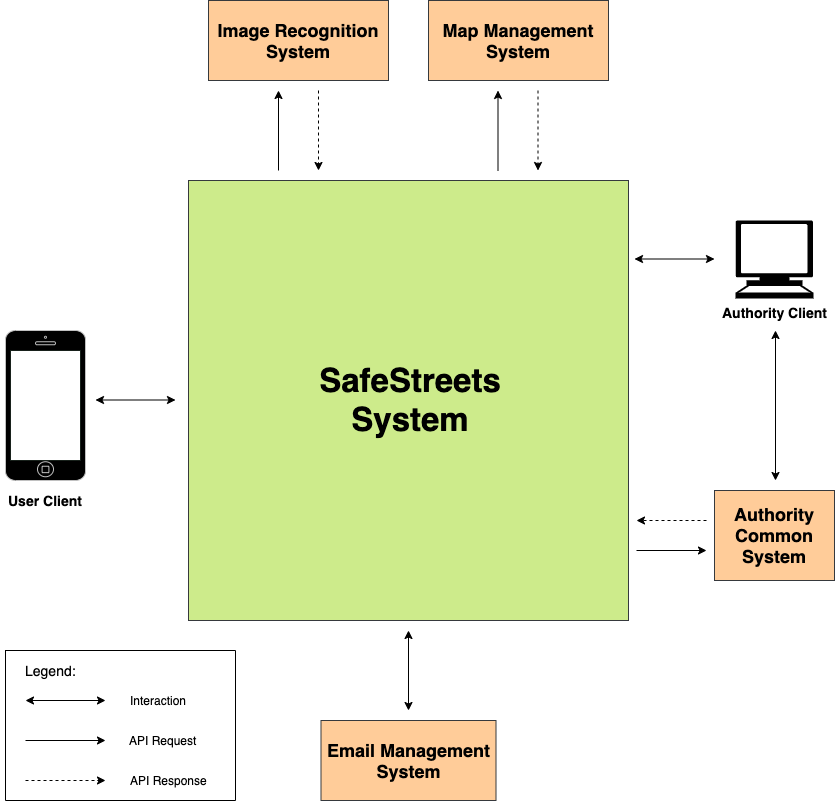
\includegraphics[scale=0.4]{contextViewPoint.png}
				\caption{\label{fig:contextViewpoint} Context Viewpoint}
			\end{figure}
		
			Now that we know which are the systems that needed, before seeing which are the modules that will consider the communication with each of them let's understand first for which functionality they are used for. The following table lists the three types of functionalities and a tick (\xtick) is used to express that the functionality needs the external systems services in order to be realized.
			
			\begin{center}
				\scalebox{0.64}{
					\begin{tabular}{|c|c|c|c|c|}
						\hline
						\diagbox{\textbf{Functionality}}{\textbf{System}} & Image Recognition & Map Management & Email Management & Authority Common \\ \hline
						Access & & & \xtick & \\ \hline
						Core & \xtick & \xtick & & \\ \hline
						Basic & & \xtick & & \\ \hline
						Advanced & & \xtick & & \xtick \\ \hline
					\end{tabular}
				} \captionof{table}{\label{tab:functionalityTable} System Mapping Table}
			\end{center}
		
		\subsubsection[Composition Diagram]{\hyperlink{toc}{Composition Diagram}}
			\label{sec:compositionDiagram}
			
			With the definition of the systems used by SafeStreets we are now able to highlight the modules used by our system in order to benefit of their services. In the following diagram we divide the system in three different types of areas, each one containing the modules considered critical for that competence.
			
			\newpage
			
			\begin{figure}[ht]
				\centering
				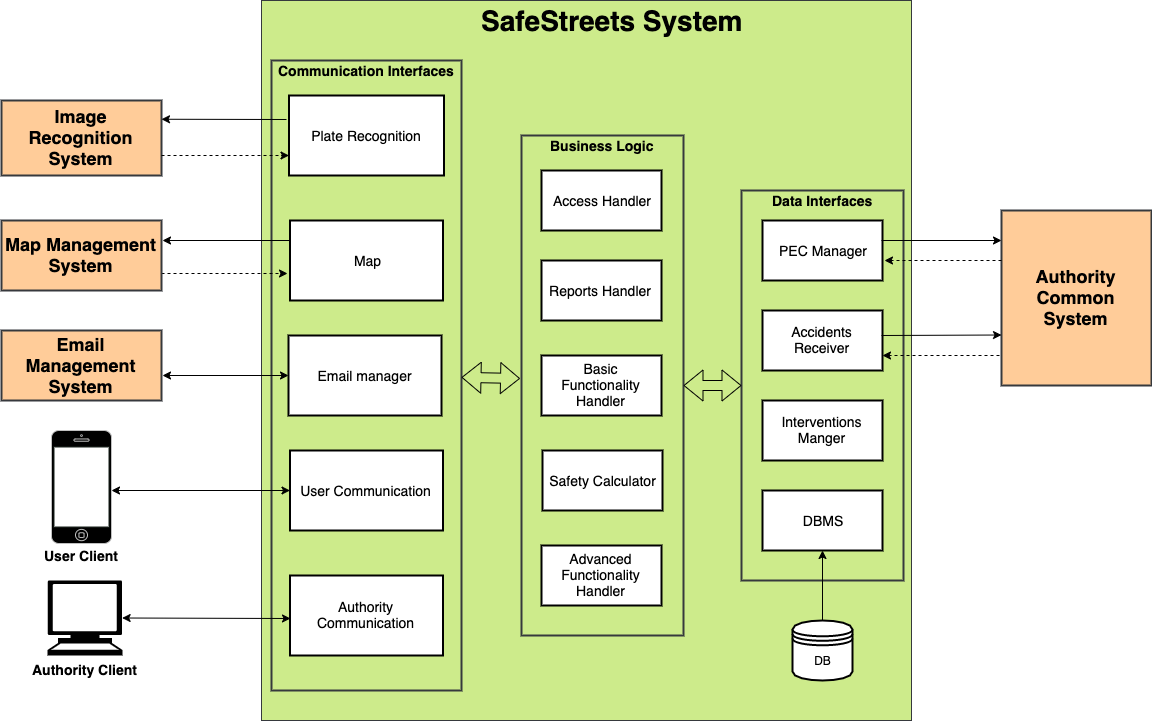
\includegraphics[scale=0.3]{compositionViewPoint.png}
				\caption{\label{fig:compositionDiagram} Composition Diagram}
			\end{figure}
		
			As we see can see in the picture above, the system is composed of three areas, each one specialized on a particular behaviors.
			
			\paragraph{Communication Interfaces} Are the interfaces that allows our system to interact with externally active agents or systems that provide services needed by the business logic. In fact, as we notice in the left hand-side of the diagram we have:
			
			\begin{itemize}
				\item \textbf{Image Recognition System:} provides thanks to an interface the methods to deal with the recognition of the plate of the vehicles
				\item \textbf{Map Management System:} provides thanks to an interface the methods to deal with all the issues related to the geographical positioning and map interaction
				\item \textbf{Email Management System:} provides the minimal email services that SafeStreets needs to consider in order to provide the recovery of the credentials and more important the recognition of the authorities
				\item \textbf{User Client:} is the client used by a user in order to benefit of SafeStreets functionalities
				\item \textbf{Authority Client:} is the client used by an authority in order to benefit of SafeStreets functionalities
			\end{itemize}
		
			All the modules defined here will bring inside the system all the services and requests coming from the outside as the ones in the business modules can process them and provide the functionalities of SafeStreets
			
			\paragraph{Business Logic} Now we have the modules that are thought to deal with the functionalities that the system has to provide. As we can see also in this case, we have a correspondence between the functionalities described in the previous section and the modules now listed:
			
			\begin{itemize}
				\item Access Handler
				\item Reports Handler
				\item Basic Functionality Handler
				\item Safety Calculator
				\item Advanced Functionality Handler
			\end{itemize}
		
			\paragraph{Data Interfaces} These last interface instead are separated from the initial ones because they provide a way to the system to access external data he needs to use in order to provide its functionalities. As we can see in the right hand-side of the diagram we only have the \textbf{Authority Common Interface} that provides the methods to retrieve all the data of the accidents that took place in a certain city and the list of all the PEC addresses of the authorities.
		
	\subsection[Component View]{\hyperlink{toc}{Component View}}
		\label{sec:componentView}
		
		\begin{figure}[ht]
			\centering
			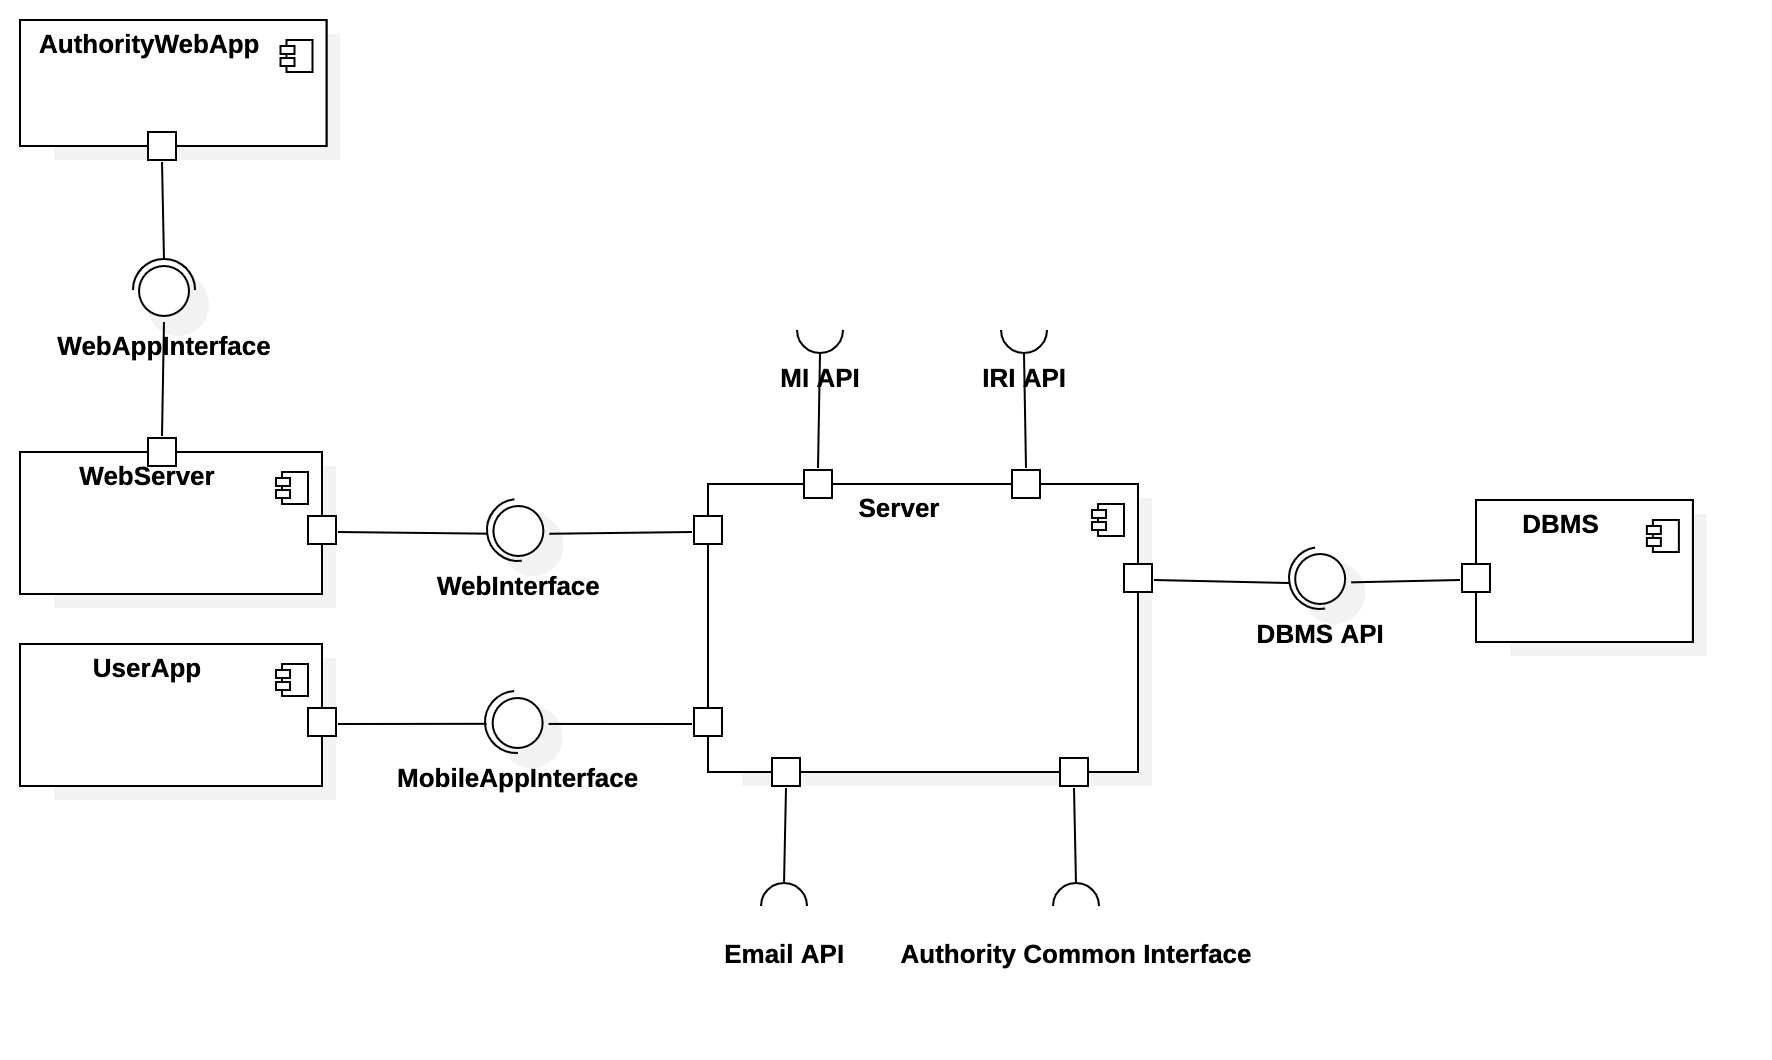
\includegraphics[scale=0.18]{/diagrams/components/highLevel.png}
			\caption{\label{fig:highLevelComp} High Level Component Diagram}
		\end{figure}
	
		With the high-level description of the system provided in the previous sections we are now able to determine which are the components that will be considered in the architecture in order to accomplish the functionalities that each of the modules identified are going to provide. In fact it is straightforward the mapping between the component diagram (\autoref{fig:compositionDiagram}) and the picture above (\autoref{fig:serverComp}). The \textbf{communication interfaces} area is mapped with all the interfaces provided by the components that provide or receive services from the outside; the \textbf{business logic} is realized by the server component where all the computation to provide the functionalities of the system takes place, while the \textbf{data interfaces} are the ones that allow the system with both the DBMS and the authority common interface.\\
		
		Before describing in detail the most important components of the system it is now the moment to precisely describe what are the components presented in this picture and what are the services provided by the interfaces:
		
		\begin{itemize}
			\item \textbf{Server:} it is the business logic of the entire system. Inside this component, that will be precisely described in the next section, takes place all the computation that allows to provide the customers the functionalities that SafeStreets has defined as its goals. The two interfaces provided by this components are the ones that allow the client systems to benefit of these functionalities, considering to have both a mobile application and a web app we need one interface directly for the mobile software while another interface for the web server that will provide to the browser of the authority the functionalities offered.
			
			\item \textbf{Web Interface:} it is the interface that allows the web server to access the methods that provide the functionalities once a request arrives from an authority.
			
			\item \textbf{Web Server:} it is the component that deals with all the issues related to the realization of a web app that needs to be displayed on the browser of the authority. In fact it provides and interface that  represents the endpoint where the browsers can access the system's functionalities.
			
			\item \textbf{Web App Interface:} it is the interface that allows the browsers to benefit of the services of SafeStreets with a web app technology.
			
			\item \textbf{Authority Web App:} it is the component that represents the browser used by the authority whenever it decides to access the system.
			
			\item \textbf{Mobile App Interface:} it is the interface that allows the mobile applications to access the functionalities provided by our system.
			
			\item \textbf{User App:} it is the component that represents the mobile software installed in the users' devices which accesses the services of SafeStreets thanks to the interface just presented.
			
			\item \textbf{MI API:} it is the interface that provides the methods to the system in order to deal with the map and geographical issues:
				\begin{itemize}
					\item Allows to retrieve the street providing a GPS position
					\item Allows to retrieve the best possible path between two positions
					\item Allows to display the colored map for the safety functionality
				\end{itemize}
			
			\item \textbf{IRI API:} it is the interface that provides the methods to the system in order to deal with the recognition of the plate of a vehicle. Remember that the algorithms accessible from this API can be helped with the information provided by the user about the plate's number and, more important, they always "have the last word": this means that whenever a result is found for the plate it will be considered correct and storable by the system; in all the cases when no result is found by the algorithms the notification will be discarded.
			
			\item \textbf{Email API:} it is the interface that provides the methods to the system in order to deal with the minimal email sending and receiving needed. An email system in fact is necessary both for the process of code verification to recognize the authorities and also for the credential recovery of both the customers
			
			\item \textbf{Authority Common Interface:} it is the interface that provides the methods to the system in order to deal with the PEC addresses and the accidents receiving. This interface is thought to be provided by a common system used by every authority where:
			
			\begin{itemize}
				\item we can retrieve all the PEC addresses of each authority, in order to do the checks in the recognition process
				\item we can retrieve all the accidents that took place in the area of an authority's competence. It is assumed that the exchange of the accidents' data develops in this way: each authority publishes its accidents on the common system as we can periodically try to retrieve thanks to this interface all the accidents that has occurred until our last check.
			\end{itemize}
		
			\item \textbf{DBMS API:} it is the interface that provides the methods to the system in order to deal with the data management process. Starting from the access one, the notification process and all the others that need to require or store information from the databases of the system (in the following section it will be clear which are the components that necessarily need to access the DBMS interface).
			 
		\end{itemize}
	
		\subsubsection[Server Component]{\hyperlink{toc}{Server Component}}
			\label{sec:serverComponent}
			
			From now on we are going to blow up the high-level component view just presented, starting with the most complex component that is the server and continuing first with its internal ones and in the end with the others that we have to take in account while defining the architecture of our system (WebServer and UserApp). In all the diagrams we are going to illustrate now the interaction between the components and the interfaces provided is carried on by means of the lollipop-socket notation. We will then continue by precisely describing each of these components to understand how they allow to obtain the functionalities of the system by providing and using the interfaces identified.\\
			
			The diagram of the next page highlights all the components that compose the server and describes both their internal and external interaction: we can see in fact the interfaces that we defined in the previous section how are provided or used by these components and how new interfaces are needed to make them interact.
			
			\begin{figure}[h!]
				\centering
				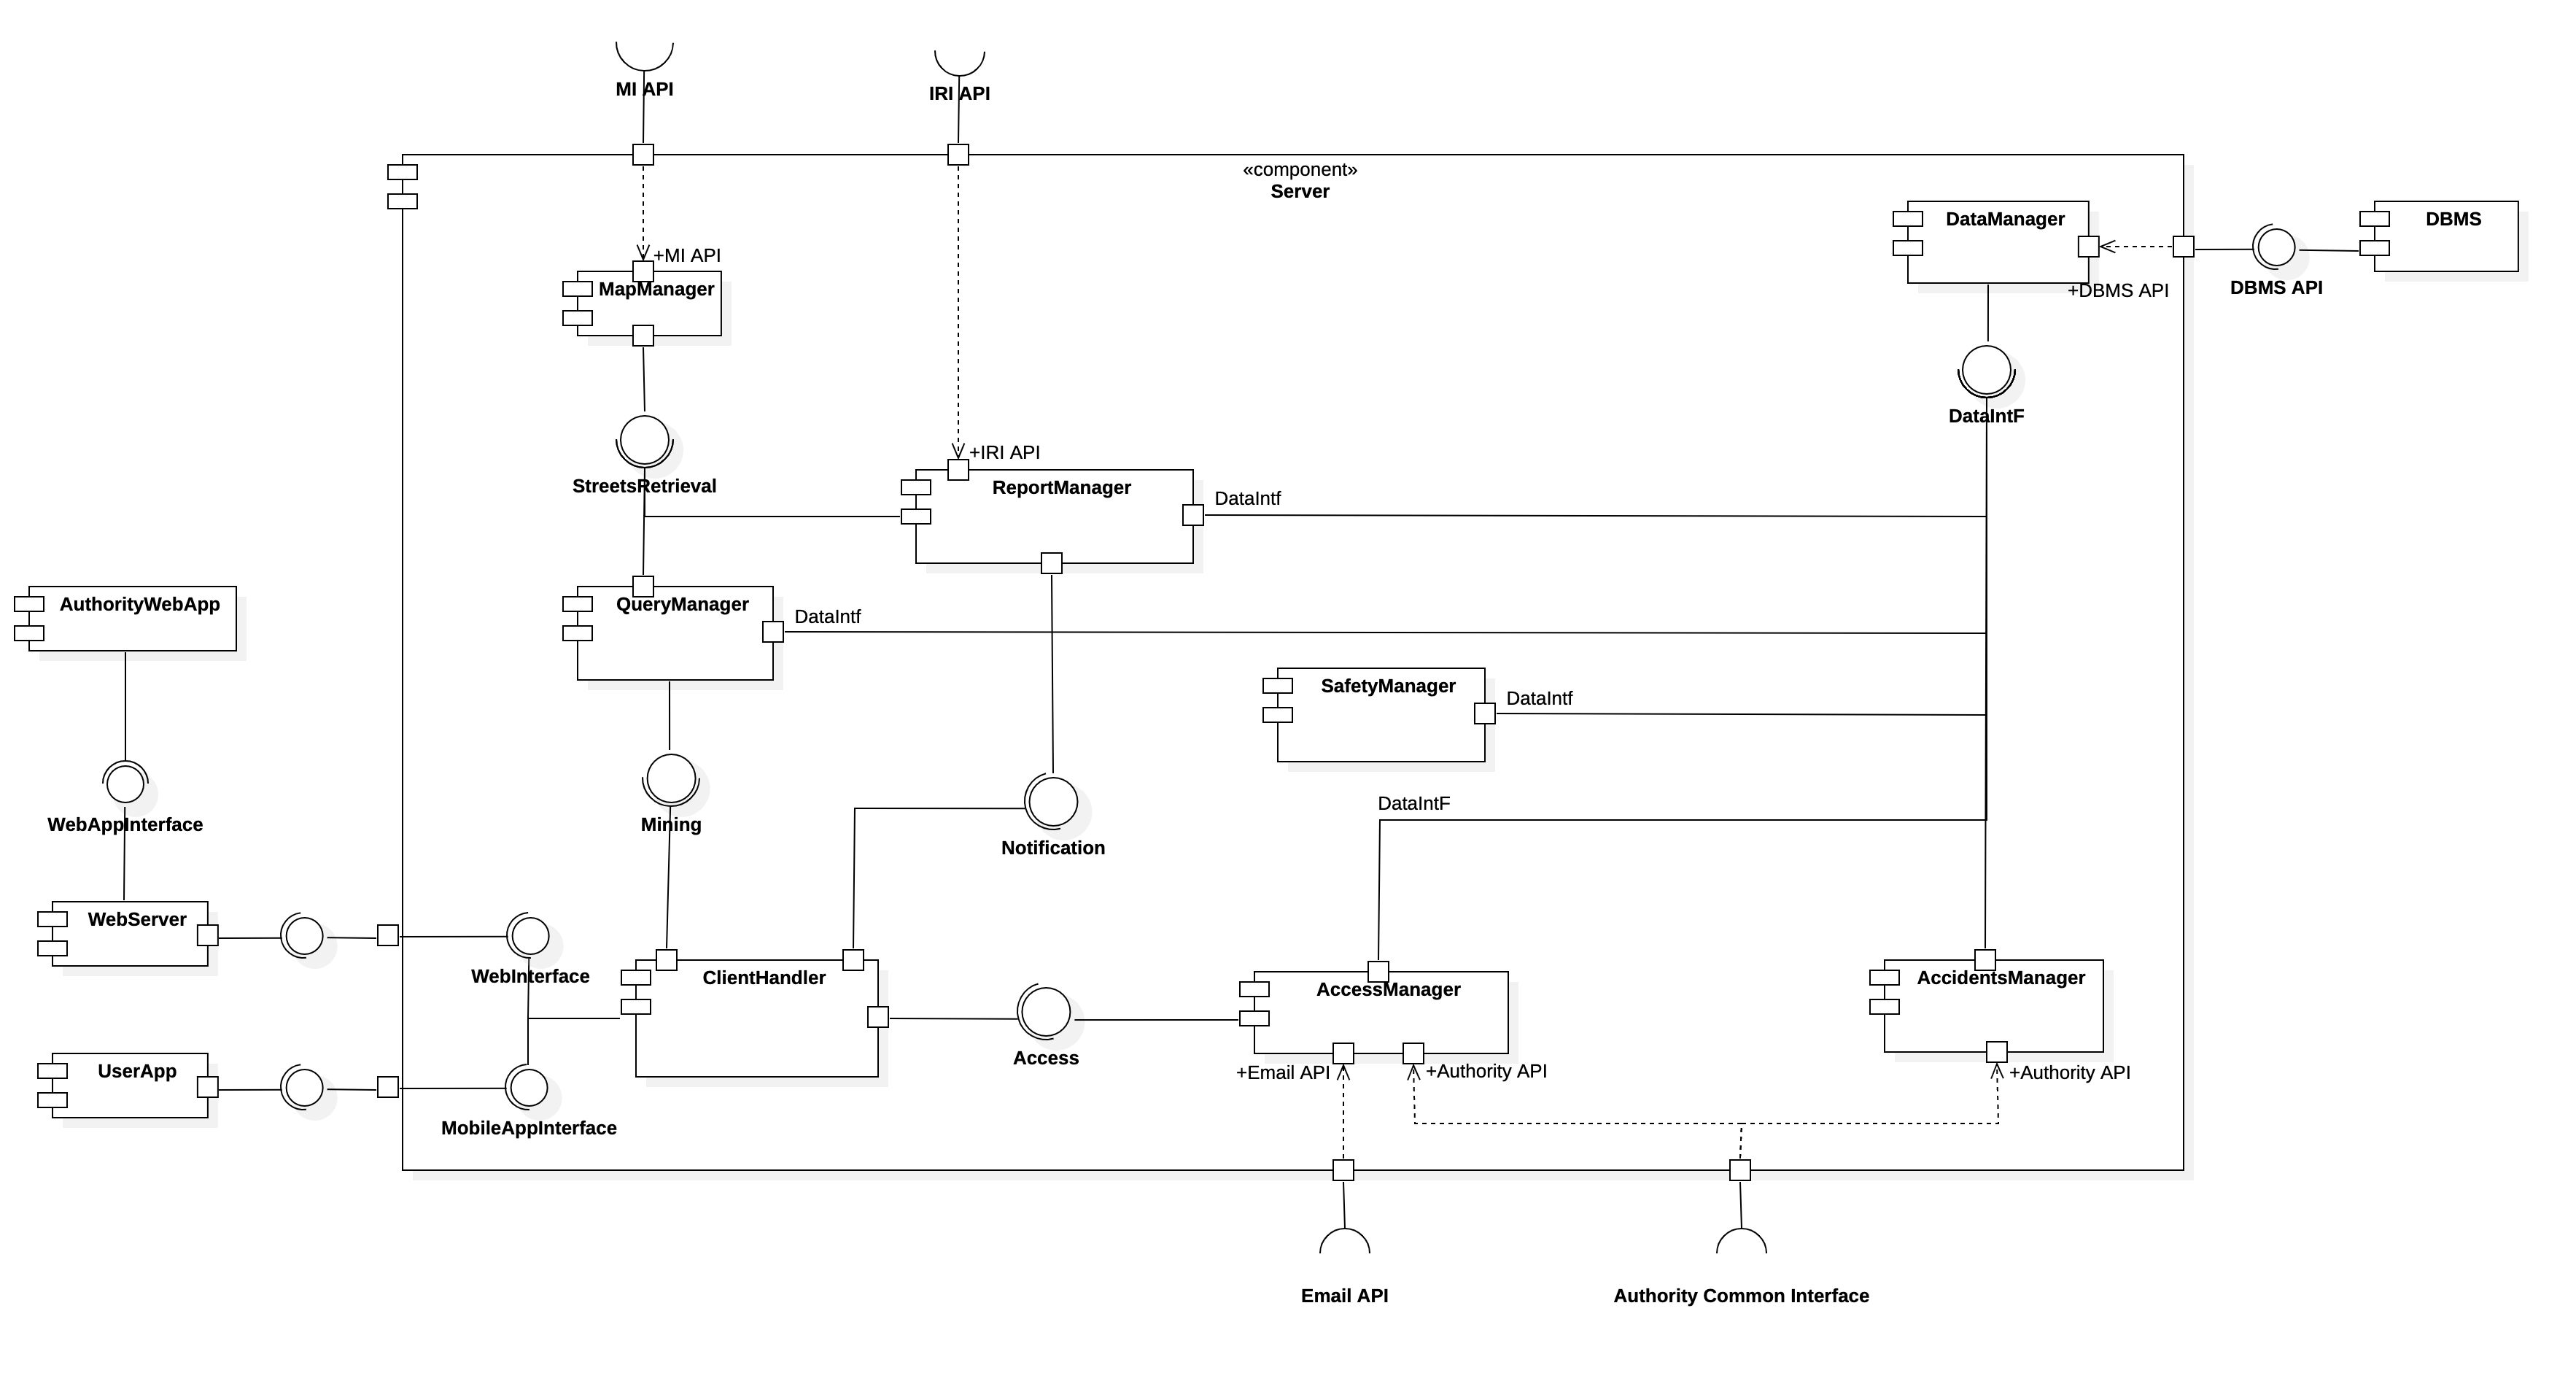
\includegraphics[scale=0.16, angle=90]{/diagrams/components/server.png}
				\caption{\label{fig:serverComp} Server Component Diagram}
			\end{figure}
		
			\FloatBarrier 
		
		\subsubsection[Client Handler Component]{\hyperlink{toc}{Client Handler Component}}
			\label{sec:clientHandlerComponent}
			
			The \emph{ClientHandler} (\autoref{fig:clientHandlerComp}) is the component that manages all the requests coming from the customers. As we see two interfaces are provided, one for the mobile application (\textbf{MobileAppInterface}) and the other for the web server that manages the web application (\textbf{WebInterface}). These two interfaces are the ones that provide the result of each request once it has been managed by the logic of the system that starts to compute in this component.
			
			\begin{figure}[h!]
				\centering
				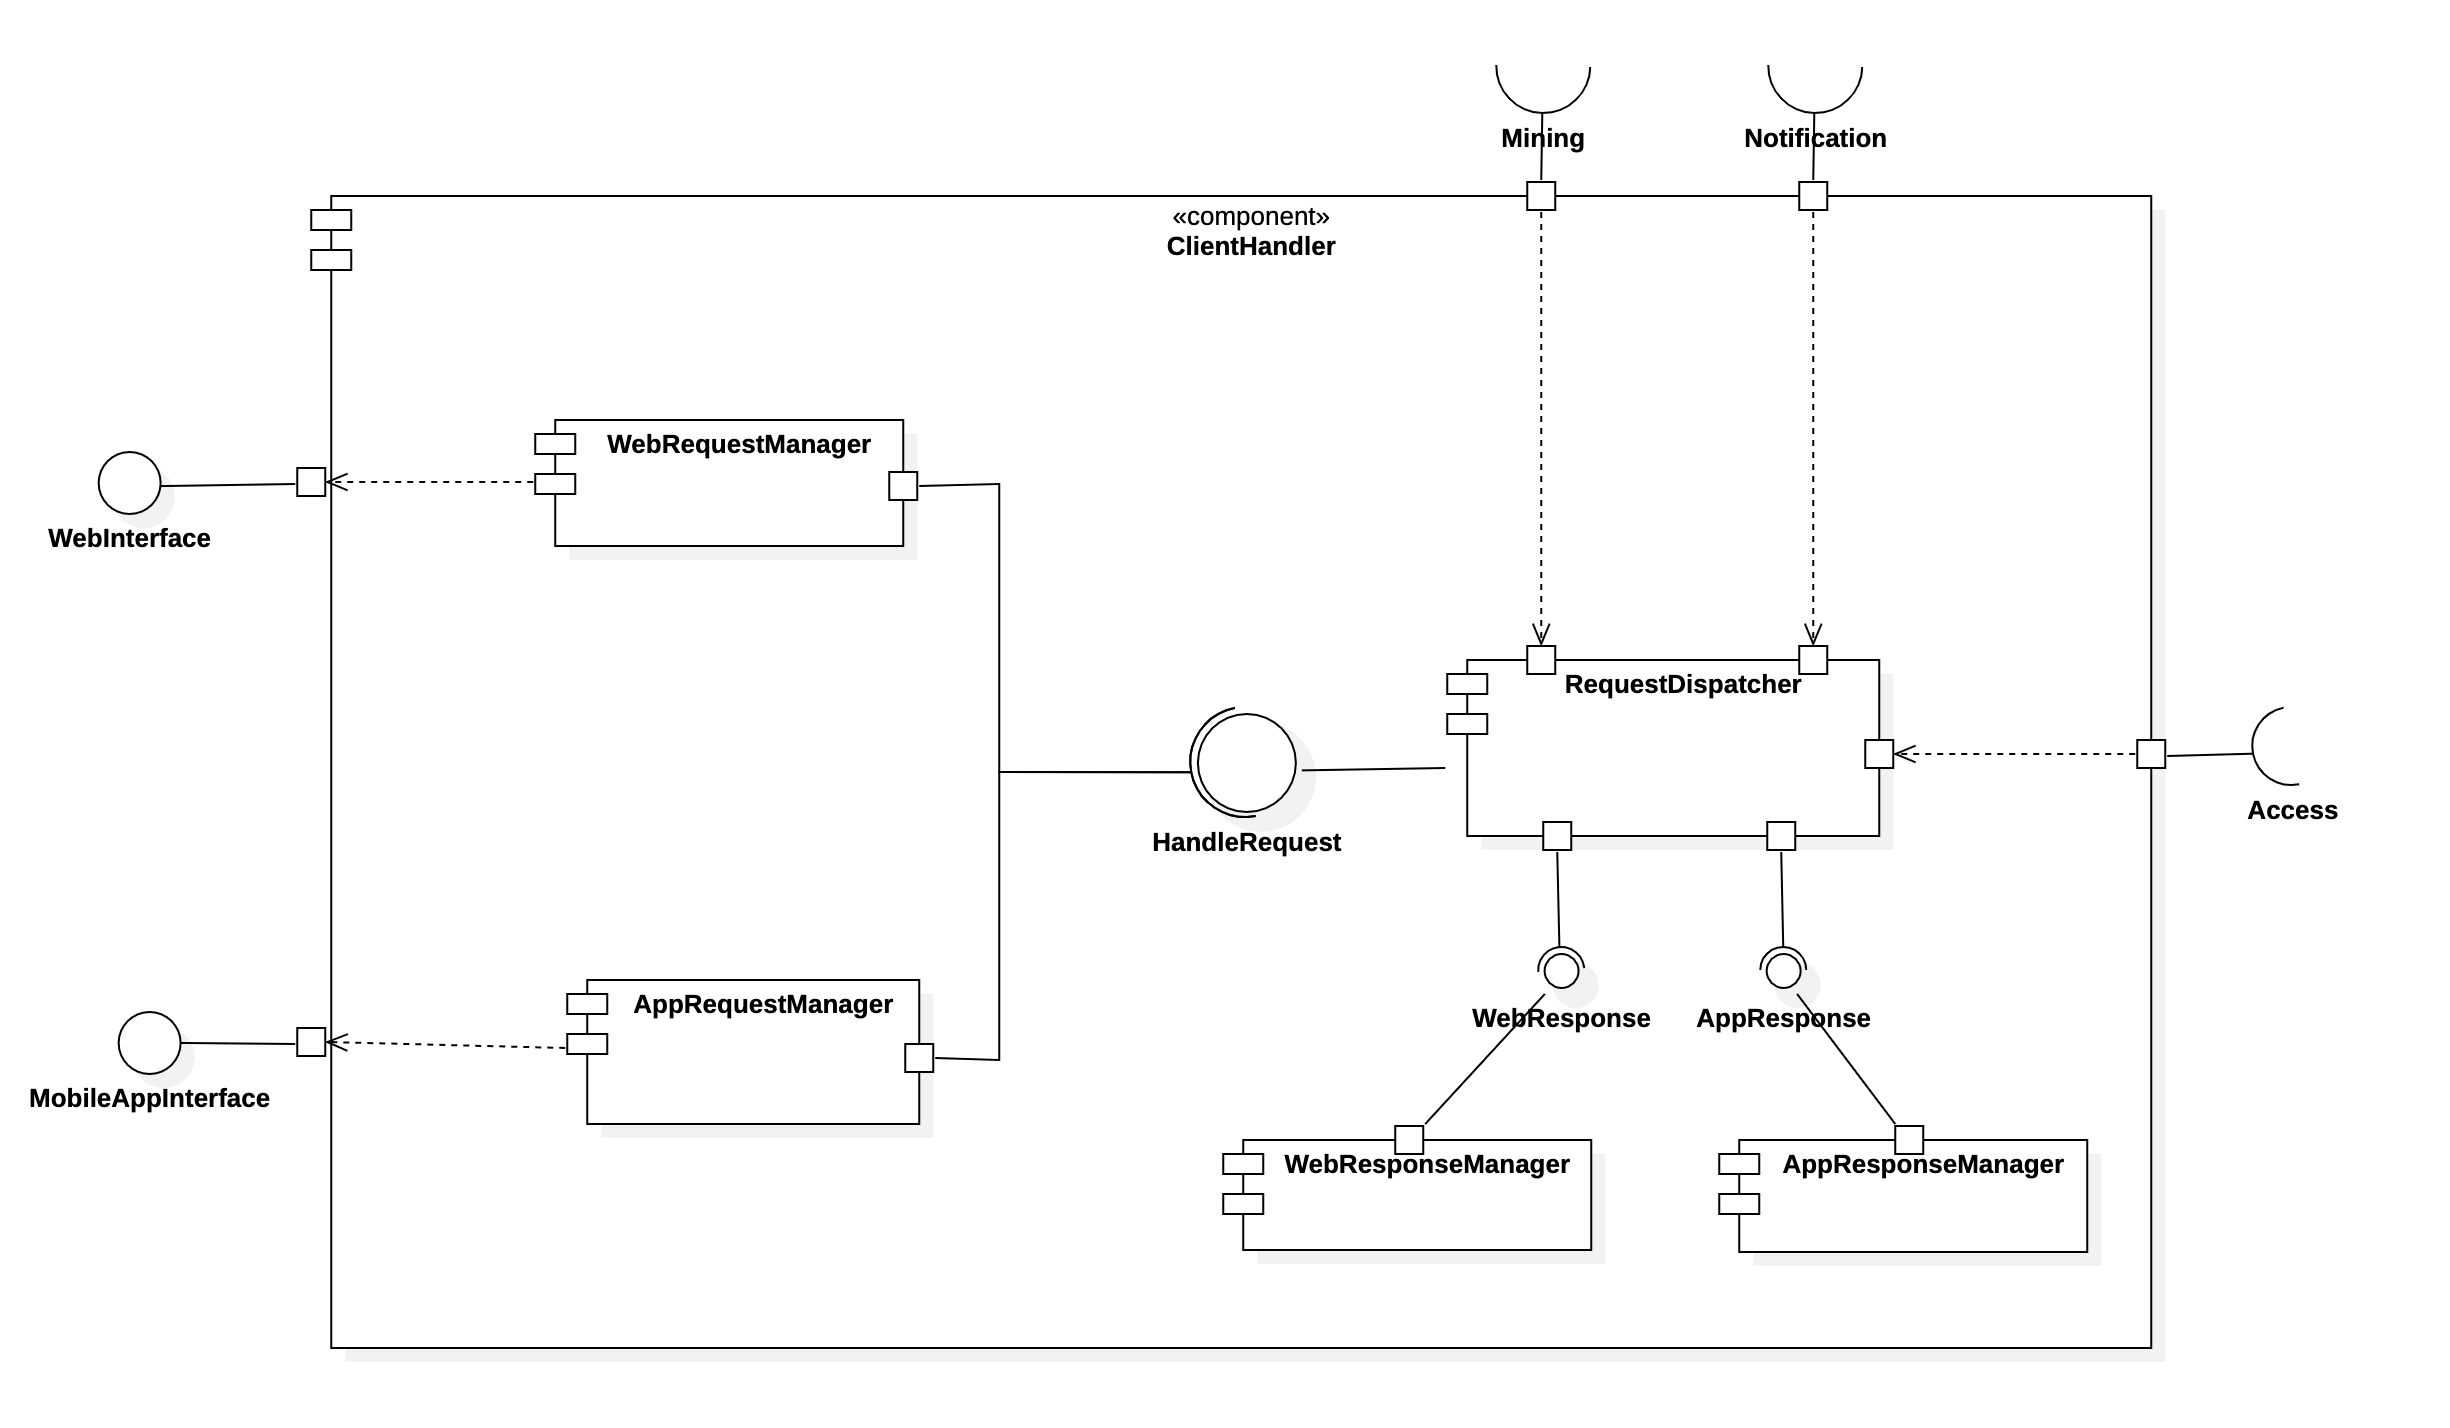
\includegraphics[scale=0.15]{/diagrams/components/clientHandler.png}
				\caption{\label{fig:clientHandlerComp} Client Handler Component Diagram}
			\end{figure}
			
			The components that allow the \emph{ClientHandler} to process a request, first receiving it and then dispatching it to the related functionality are:
			
			\begin{itemize}
				\item \textbf{WebRequestManager:} it is the component that manages all the requests that come from the web application, hence from the web server that uses the \textbf{WebInterface} realized by this component.
				
				\item \textbf{AppRequestManager:} it is the component that manages all the requests that come from the mobile application, hence from the device that uses the \textbf{MobileAppInterface} realized by this component.
				
				\item \textbf{RequestDispatcher:} it is the component that allows to handle each type of request that comes either from the web app or the mobile one. In fact, thanks to the \textbf{HandleRequest Interface} the components previously described can deploy the request to this one that, depending on the type of the request will need to use different services in order to provide the functionality it is requiring. In fact, as we can see there are several interfaces that are used by this component:
				
				\begin{itemize}
					\item \textbf{Mining Interface:} allows to benefit of the methods provided by the \emph{QueryManager} component that is the one which manages all the queries related to the basic and the advanced functionalities.
					
					\item \textbf{Notification Interface:} it is the interface that allows to manage the notification process once a request to report a parking violation is received by a user.
					
					\item \textbf{Access Interface:} it is the interface that allows to deal with all the issues related to the access to the system. This means: the login, the registration, the credential recovery, the recognition of the authorities...
					
					\item \textbf{WebResponse Interface:} it is the interface that allows to process the information received from the logic of the system as it can be used by the \emph{WebServer} to be displayed on the web app.
					
					\item \textbf{MobileResponse Interface:} it is the interface that allows to process the information received from the logic of the system as it can be used by the device to be displayed on the mobile app.
				\end{itemize}
			\end{itemize}
		
		\subsubsection[Access Manager Component]{\hyperlink{toc}{Access Manager Component}}
			\label{sec:accessManagerComponent}
			
			The \emph{AccessManager} (\autoref{fig:accessManagerComp}) is the component that manages all the issues related to the access of the customers to the system. As we have said several times when defining the goals and requirements of SafeStreets, in fact, it is fundamental to recognize the clients and thus to provide a registration process.\\
			
			The components described in the following diagram are the ones that allow to provide the access functionalities of:
			
			\begin{itemize}
				\item Registration
				\item Login
				\item Credentials Recovery
			\end{itemize}
		
			In order to provide the methods that allow to realize these functionalities through the \textbf{Access Interface}, this component has also to benefit of the external services provided by the methods of the \textbf{Email API} and \textbf{Authority API}. The interface that allows to access and manage the data stored in the system is obviously fundamental for all the checks needed and to store new customers in the application.\\
			
			The components that allow the \emph{AccessManager} to process an access request, meaning one of the three functionalities listed before are:
			
			\begin{itemize}
				\item \textbf{Email Manager:} it is the component that uses the methods provided by the \textbf{Email API} in order to have a way to send the mails with the recognition code to the authorities and to offer the service of the credentials recovery by sending an email to the address that requests for recovering its password. This component provides the \textbf{mail Interface} that is used by the other components that realizing these functionalities have to deal with the email system.
			
				\item \textbf{PEC Manager:} it is the component that deals with all the issues related to the PEC addresses of the authorities. In fact it uses the methods provided by the \textbf{Authority API} in order to know which are the existing addresses of all the authorities and then uses the \textbf{mail Interface} to provide through the \textbf{PEC Interface} the methods that allow to send the verification code in the registration process.
			\end{itemize}
			
			\begin{figure}[ht]
				\centering
				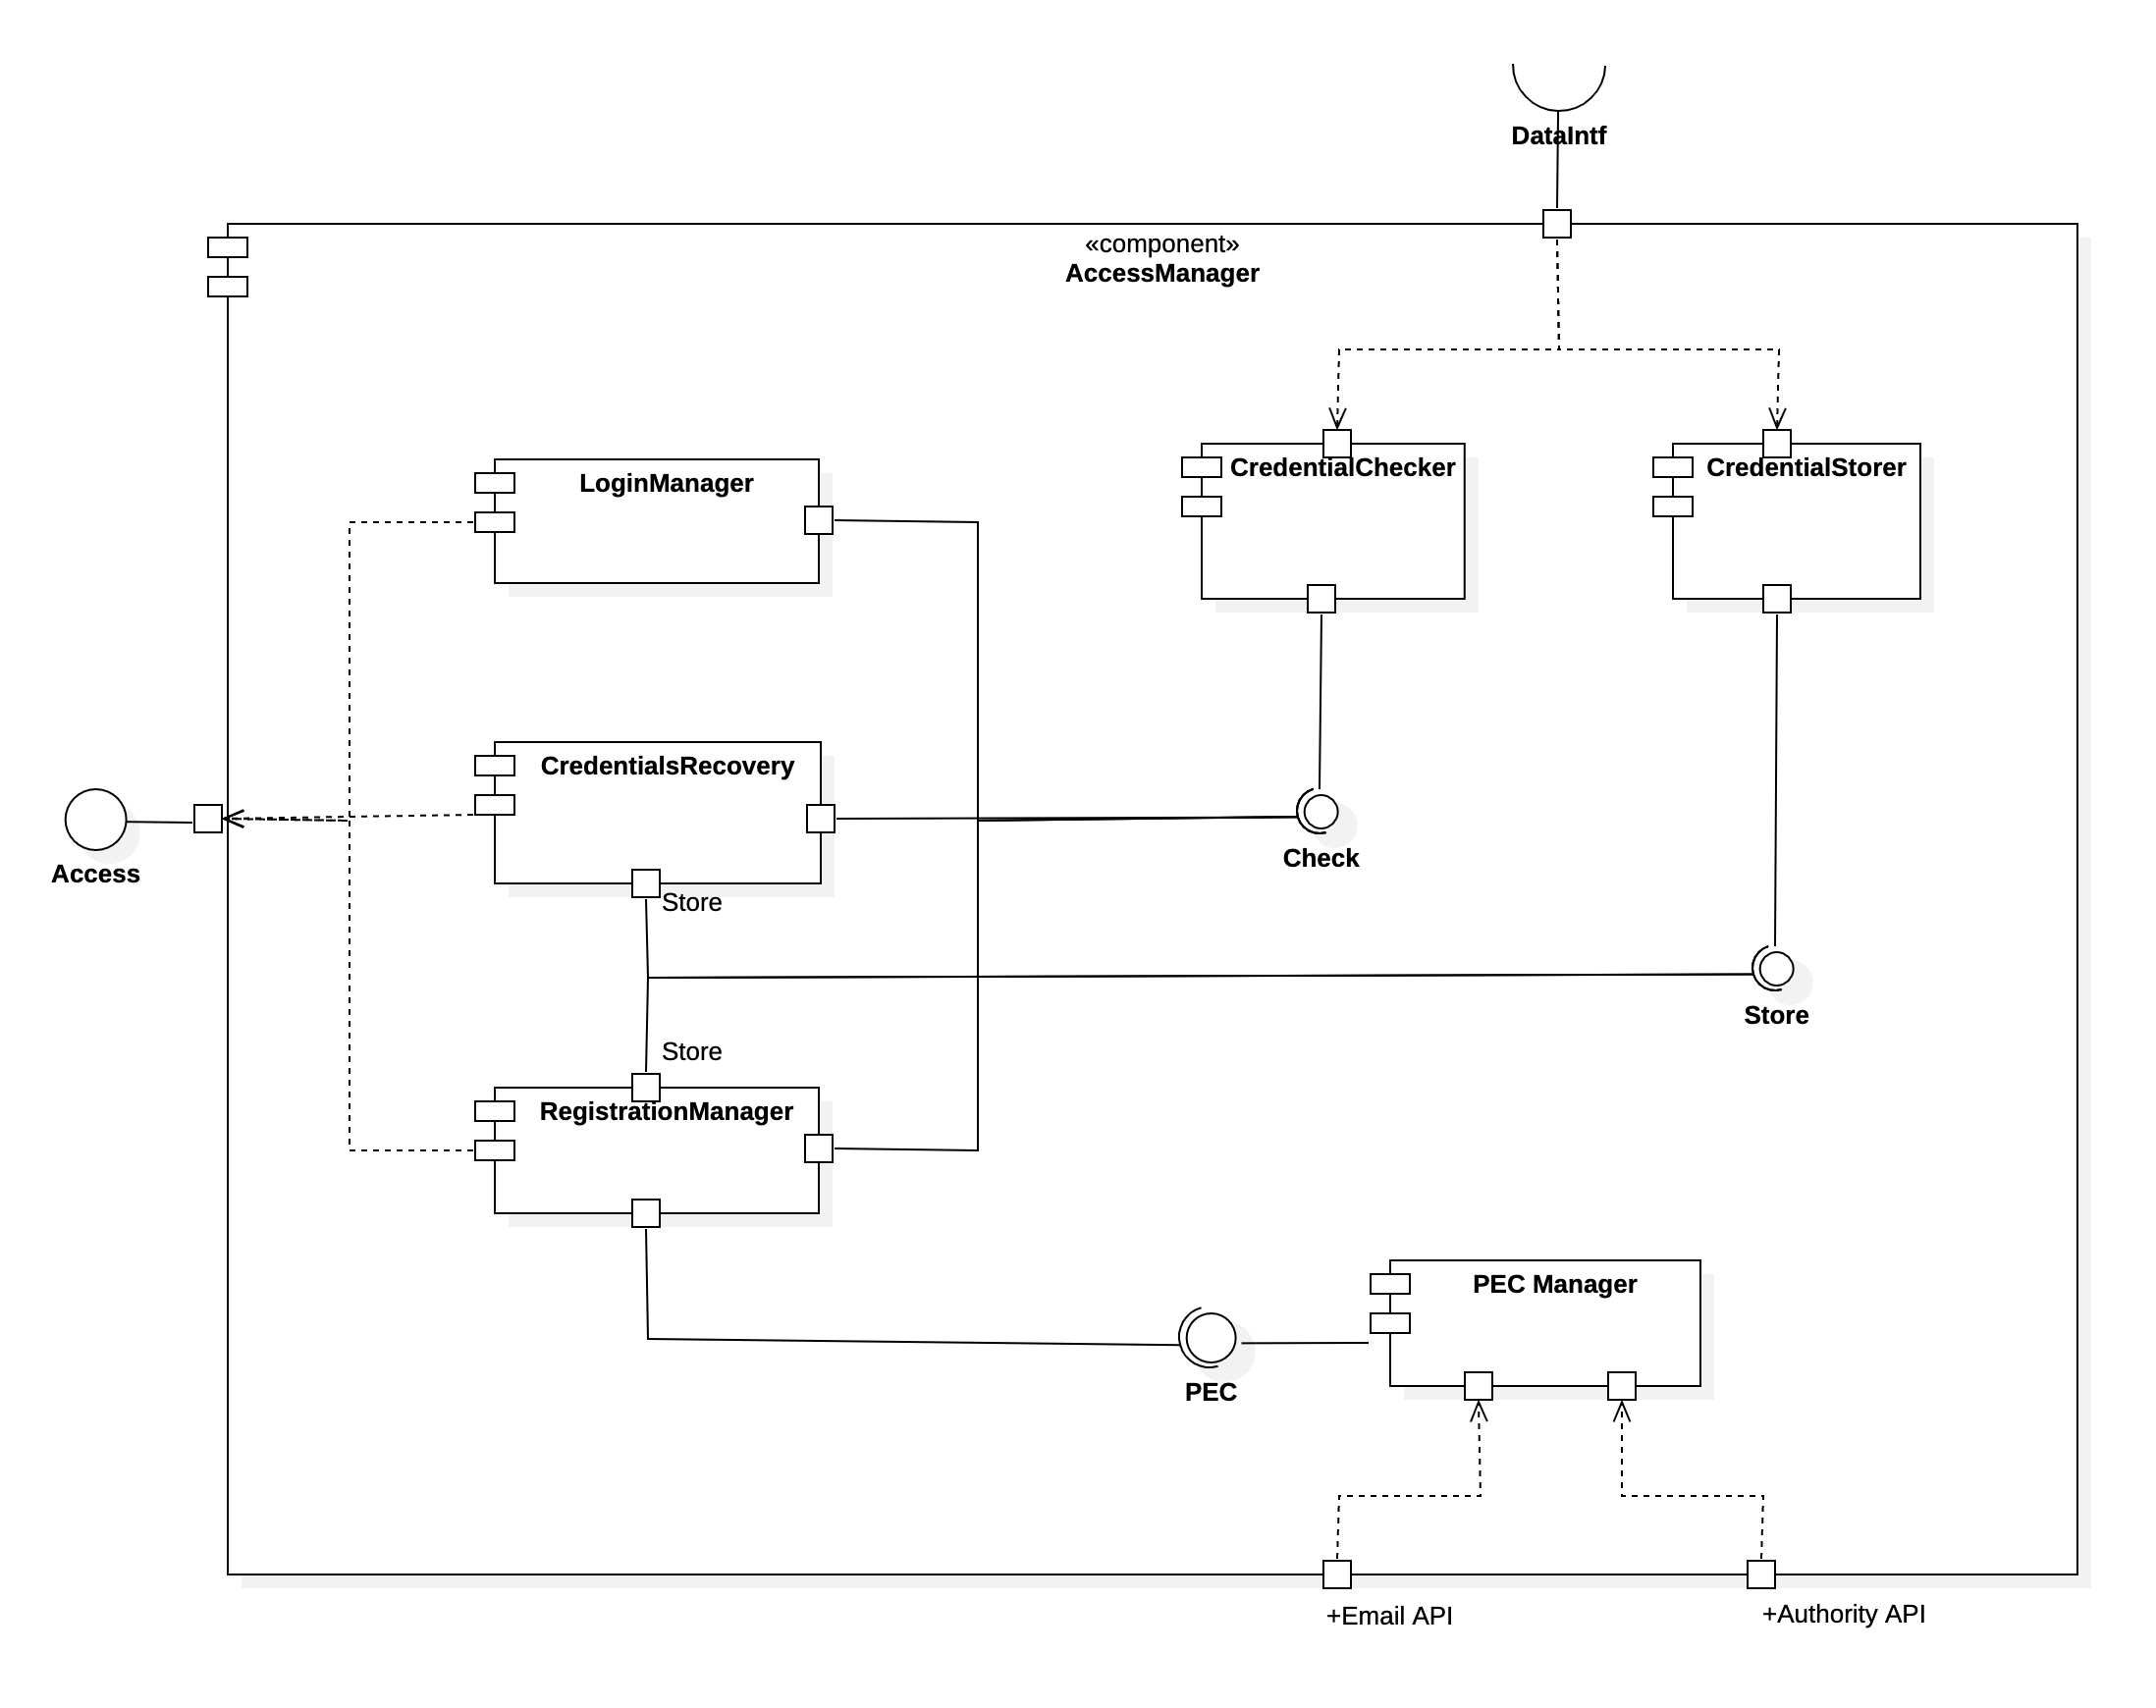
\includegraphics[scale=0.16]{/diagrams/components/accessManager}
				\caption{\label{fig:accessManagerComp} Access Manager Component Diagram}
			\end{figure}
		
			\begin{itemize}
				\item \textbf{LoginManager:} it is the component that deals with the login process. It realizes the \textbf{Access Interface} by providing the methods for the login and has always to interact with the \emph{CredentialChecker} component in order to verify the credentials of the logging customer. In this way, thanks to the \textbf{Check Interface}, this component will control the credential of either the user or the authority and decide if to authenticate them or not.
				
				\item \textbf{CredentialRecovery:} it is the component that deals with the credentials recovery process. It realizes the \textbf{Access Interface} by providing the methods for the recovery and thus it needs to interact with both the \emph{CredentialChecker} and the \emph{CredentialStorer:} components. Thanks to the \textbf{Check Interface} and the \textbf{Store Interface}, in fact, it will be able to control the identity of the customer who is requiring to recover its credentials and store the new information related to the customer. Obviously the \textbf{mail Interface} is also needed in order to send the email to the customer that is requiring to recover its credentials.
				
				\item \textbf{RegistrationManager:} it is the component that deals with the registration of the customers. It realizes the \textbf{Access Interface} by providing the methods to register both the user and the authority and thus needs to use the \textbf{Check Interface} and the \textbf{Store Interface}. In fact, this component will need to check for the new credentials to be feasible and then to store the new data related to the registering customer. The \textbf{PEC Interface} is used for the authority registration process to send the verification code and check the address.
				
				\item \textbf{CredentialChecker:} it is the component that deals with all the checks needed in the access functionalities previously described by providing the \textbf{Check interface}. Obviously to perform these checks it needs to access the customers database of the system and thus the methods provided by the \textbf{DataIntF Interface}.
				
				\item \textbf{CredentialStorer:} it is the component that deals with the storing of all the data used in the access functionalities previously described by providing the \textbf{Store Interface}.
				Obviously in order to store the information in the database of the customers in the system it needs to use the methods provided by the \textbf{DataIntF Interface}
			\end{itemize}
		
		\subsubsection[Query Manager Component]{\hyperlink{toc}{Query Manager Component}}
			\label{sec:queryManagerComponent}
			
			The \emph{QueryManger} (\autoref{fig:queryManagerComp}) is the component that manages the requests related either to the basic or the advanced functionalities (see section \ref{sec:generalContext} for the precise functionalities description) coming from the customers with the realization of the \textbf{Mining Interface}. Hence, this component needs first to identify the request as it can be checked for the filters used thanks to the \textbf{Check Interface} and then, once identified the functionality, it realizes the respective query with the respective interface provided by the correct component:
			
			\begin{itemize}
				\item Interventions Interface
				\item Safety Interface
				\item Visibility Interface
				\item Dangerous Interface
				\item Frequency Interface
			\end{itemize}
		
			Once the query is ready it is prepared and sent to the component that will execute it through the \textbf{Send Interface} realized by the \emph{QuerySender}.\\
			
			The components that allow the \emph{QueryManager} to process the requests related to a functionality are:
			
			\begin{itemize}
				\item \textbf{FunctionalityIdentifier:} it is the components that realizes the \textbf{Mining Interface} by providing the methods related to the processing of a request that deals with one of the basic or advanced functionalities. This component first needs to recognize which is the functionality requested as it can check it and then prepare it to be executed. Thanks to the \textbf{Check Interface} it controls if the filters in the request are feasible with the ones related to the functionality recognized and then it calls the method that builds the query from the correct interface between the ones presented before.
			\end{itemize}
			
			\begin{figure}[ht]
				\centering
				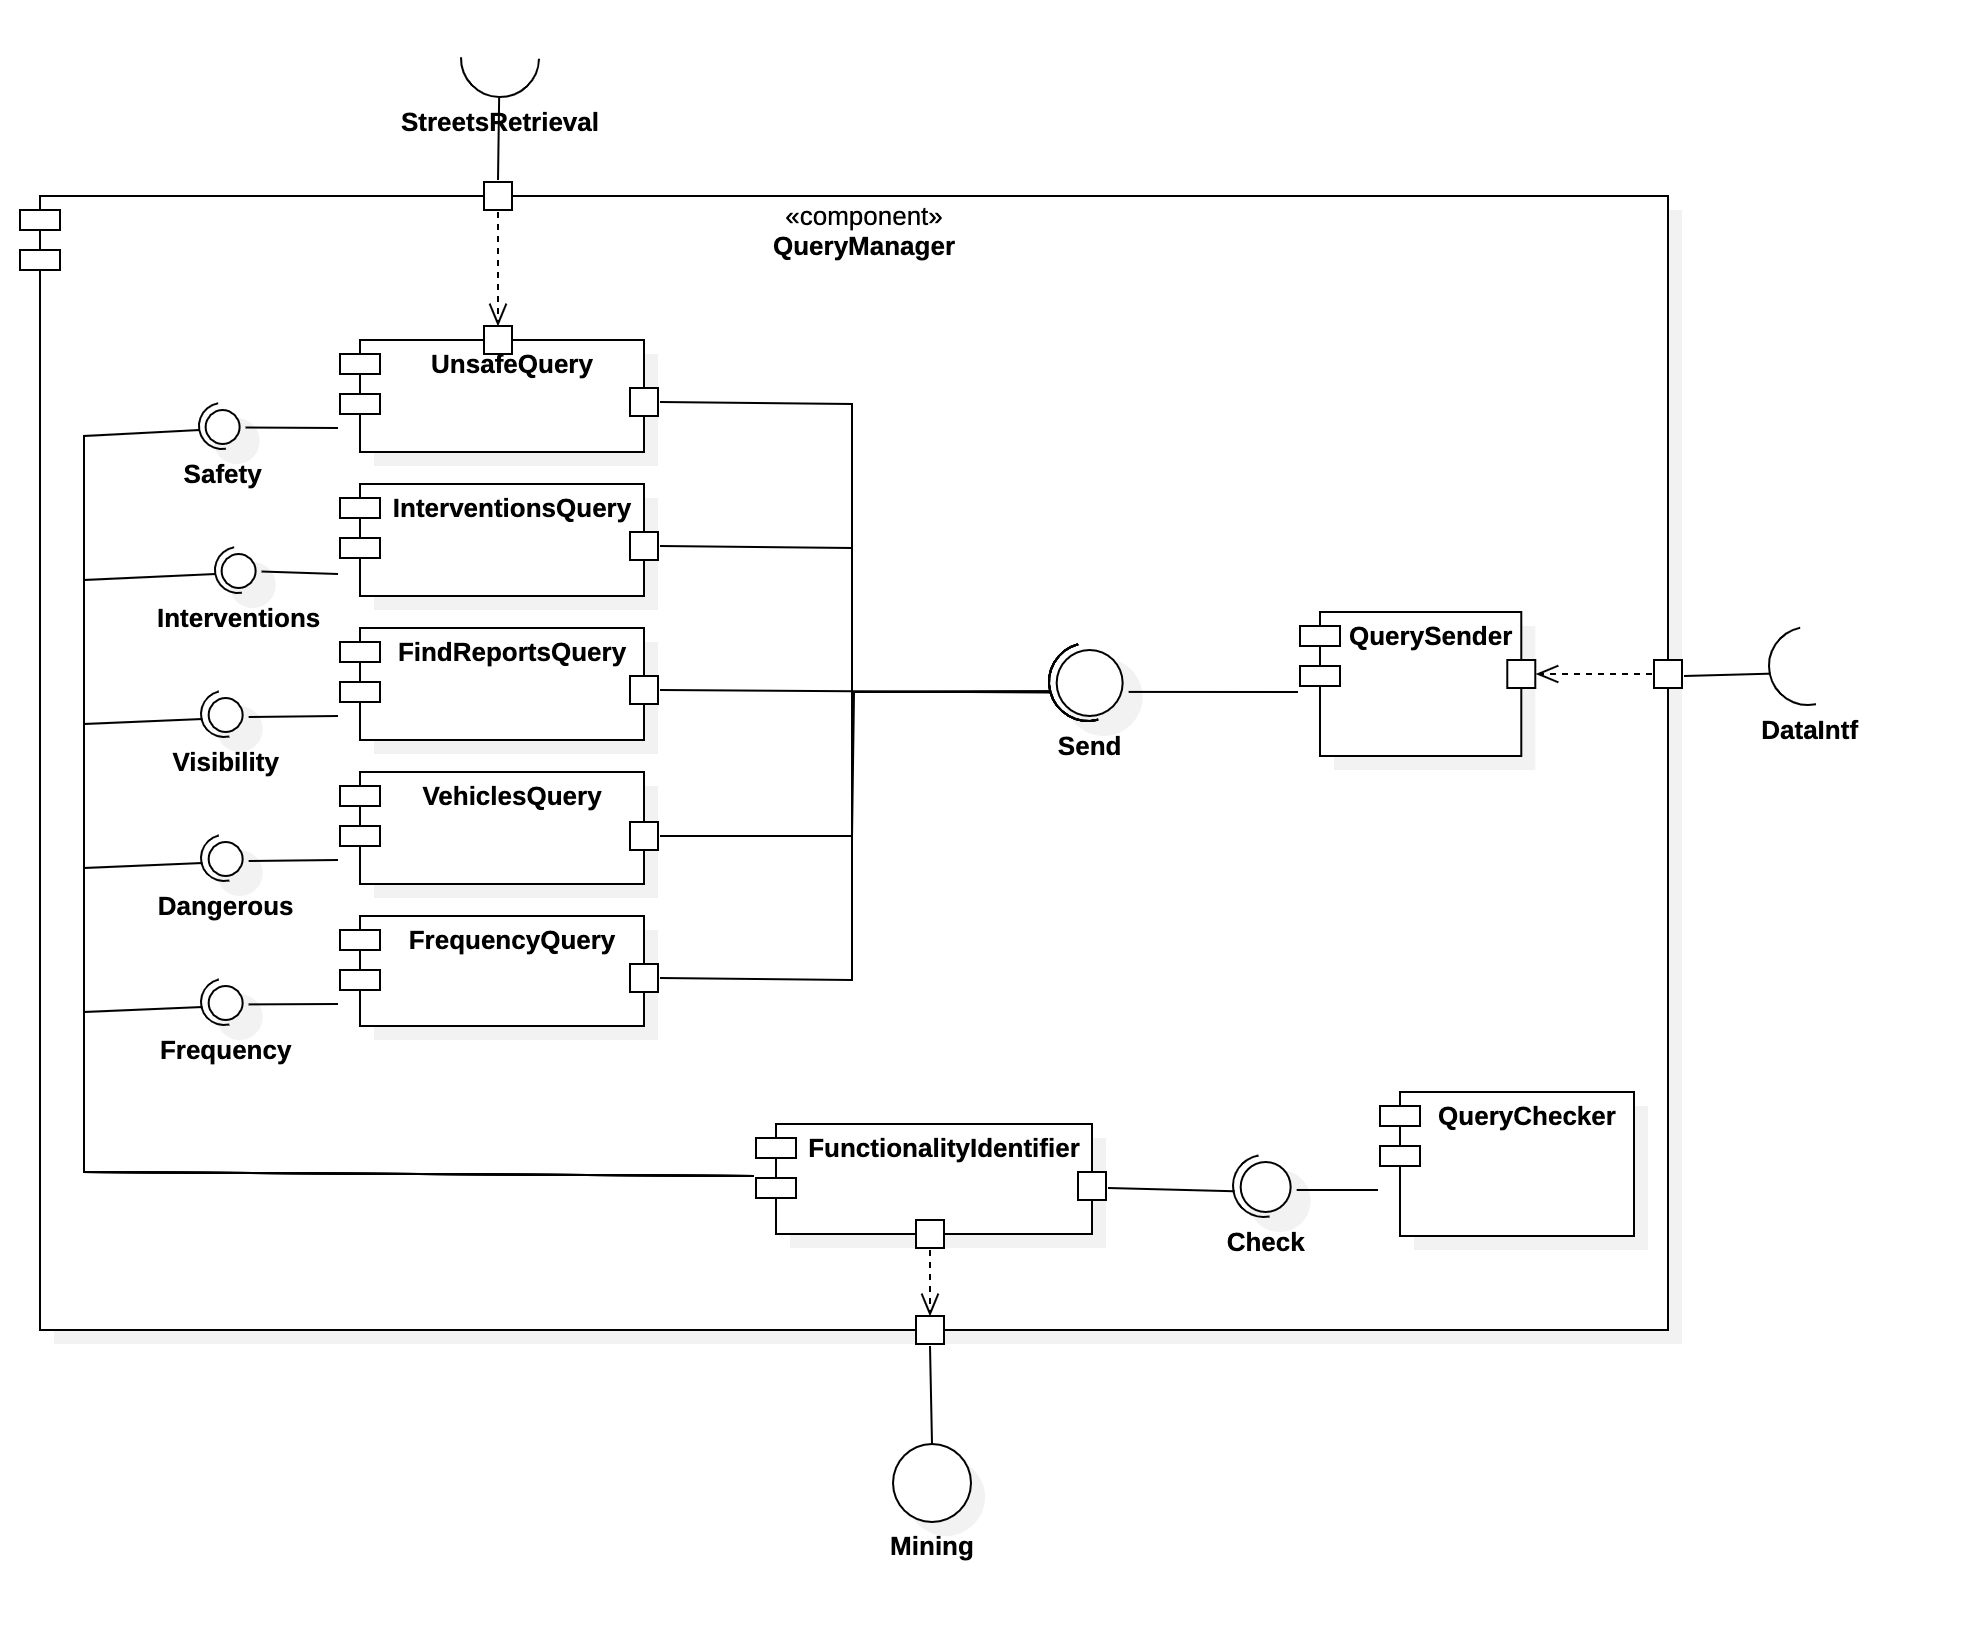
\includegraphics[scale=0.2]{/diagrams/components/queryManager.png}
				\caption{\label{fig:queryManagerComp} Query Manager Component Diagram}
			\end{figure}
		
			\begin{itemize}
				\item \textbf{UnsafeQuery:} it is the component that manages the query related to the safety functionality. Hence it will select the correct area and retrieve the safety of all the streets required by the customer as they can be displayed on the map. This component realizes the \textbf{Safety Interface} and needs to use the methods provided by the \textbf{StreetsRetrieval Interface} as it can manage the request of the customer to find the safety of the best path between the two positions he specified.
				
				\item \textbf{InterventionsQuery:} it is the component that manages the query related to suggestion for possible interventions functionality. Hence it will prepare the query over the city selected and retrieve all the suggestions for it. This component realizes the \textbf{Interventions Interface} used by the \emph{FunctionalityIdentifier}.
				
				\item \textbf{FindREportsQuery:} it is the component that manages the query related to the functionality provided only to the authorities in order to give them the most detailed level of visibility for the reported violations. This component realizes the \textbf{Visibility Interface} used by the \emph{FunctionalityIdentifier}.
				
				\item \textbf{VehiclesQuery:} it is the component that manages the query related to the dangerous vehicles functionality. Hence it will prepare the query with the filters already checked and retrieve the type of dangerous vehicles. This component realizes the \textbf{Dangerous Interface} used by the \emph{FunctionalityIdentifier}.
				
				\item \textbf{FrequencyQuery:} it is the component that manages the query related to the violations frequency functionality. Hence it will prepare the query with the filters already checked and retrieve the streets with most violations. This component realizes the \textbf{Frequency Interface} used by the \emph{FunctionalityIdentifier}.
				
				\item \textbf{QuerySender:} it is the component that allows to send the query to the \emph{DataManager} component that allows to execute it and retrieve the results. Thanks to the \textbf{Send Interface}, in fact, the five components just presented will send the query they have prepared as it can be executed over the related databases.
			\end{itemize}
		
		\subsubsection[Report Manager Component]{\hyperlink{toc}{Report Manager Component}}
			\label{sec:reportManagerComponent}
			
			The \emph{ReportManager} (\autoref{fig:reportManagerComp}) is the component that manages the notification process of the system, hence the one that we called the core functionality of SafeStreets. We have to remark that the notification process starts when a report arrives from a user and then the methods of the \textbf{Notification Interface} are invoked and ends when all the information about the report are stored in the system. At the end of the process each notification stored is marked as unread as it can be retrieved by the competent authority whenever it requires to benefit of the check unread reports functionality.\\
			
			As we have already said in the description of the functionality we will need to complete the data provided by the user with some controls and additions that will be performed thanks to the three interfaces that we can see are used by this component:
			
			\begin{itemize}
				\item StreetRetrieval Interface
				\item IRI API
				\item DataIntF Interface
			\end{itemize}
		
			The components that allow the \emph{ReportManager} to handle completely the notification process, hence the report of the user and the retrieval by the authority, are:
			
			\begin{itemize}
				\item \textbf{ReportValidator:} it is the main component that deals with the notification process of the user-side. Once a report is notified by a user, all the information related to it will be delivered to this component by the \emph{ClientHandler} thanks to the \textbf{Notification Interface}. Before storing the information it has to be managed in order to add the missing details and validate its content; these two further considerations are managed with the methods provided by the interfaces:
				
				\begin{itemize}
					\item \textbf{HandlePosition:} it is the interface that retrieves the street providing the GPS position of where the parking violation occurred.
					
					\item \textbf{PlaceRecognition:} it is the interface that retrieves the plate of the reported vehicle providing the images of the infraction and the possible additional number inserted by the user. It is important to remark once more that the result of the methods provided by this interface will determine whether to discard or not the notification.
					
					\item \textbf{Check:} it is the interface that allows to check if there exists already the same notification in the system. As we have already said, it is useless to store twice the same notification, in the case of a duplicate the current one will be discarded.
					
					\item \textbf{Store:} it is the interface that allows to store the notification once the data completion and the validity have been carried out by the component.
				\end{itemize}
			\end{itemize}
			
			\begin{figure}[ht]
				\centering
				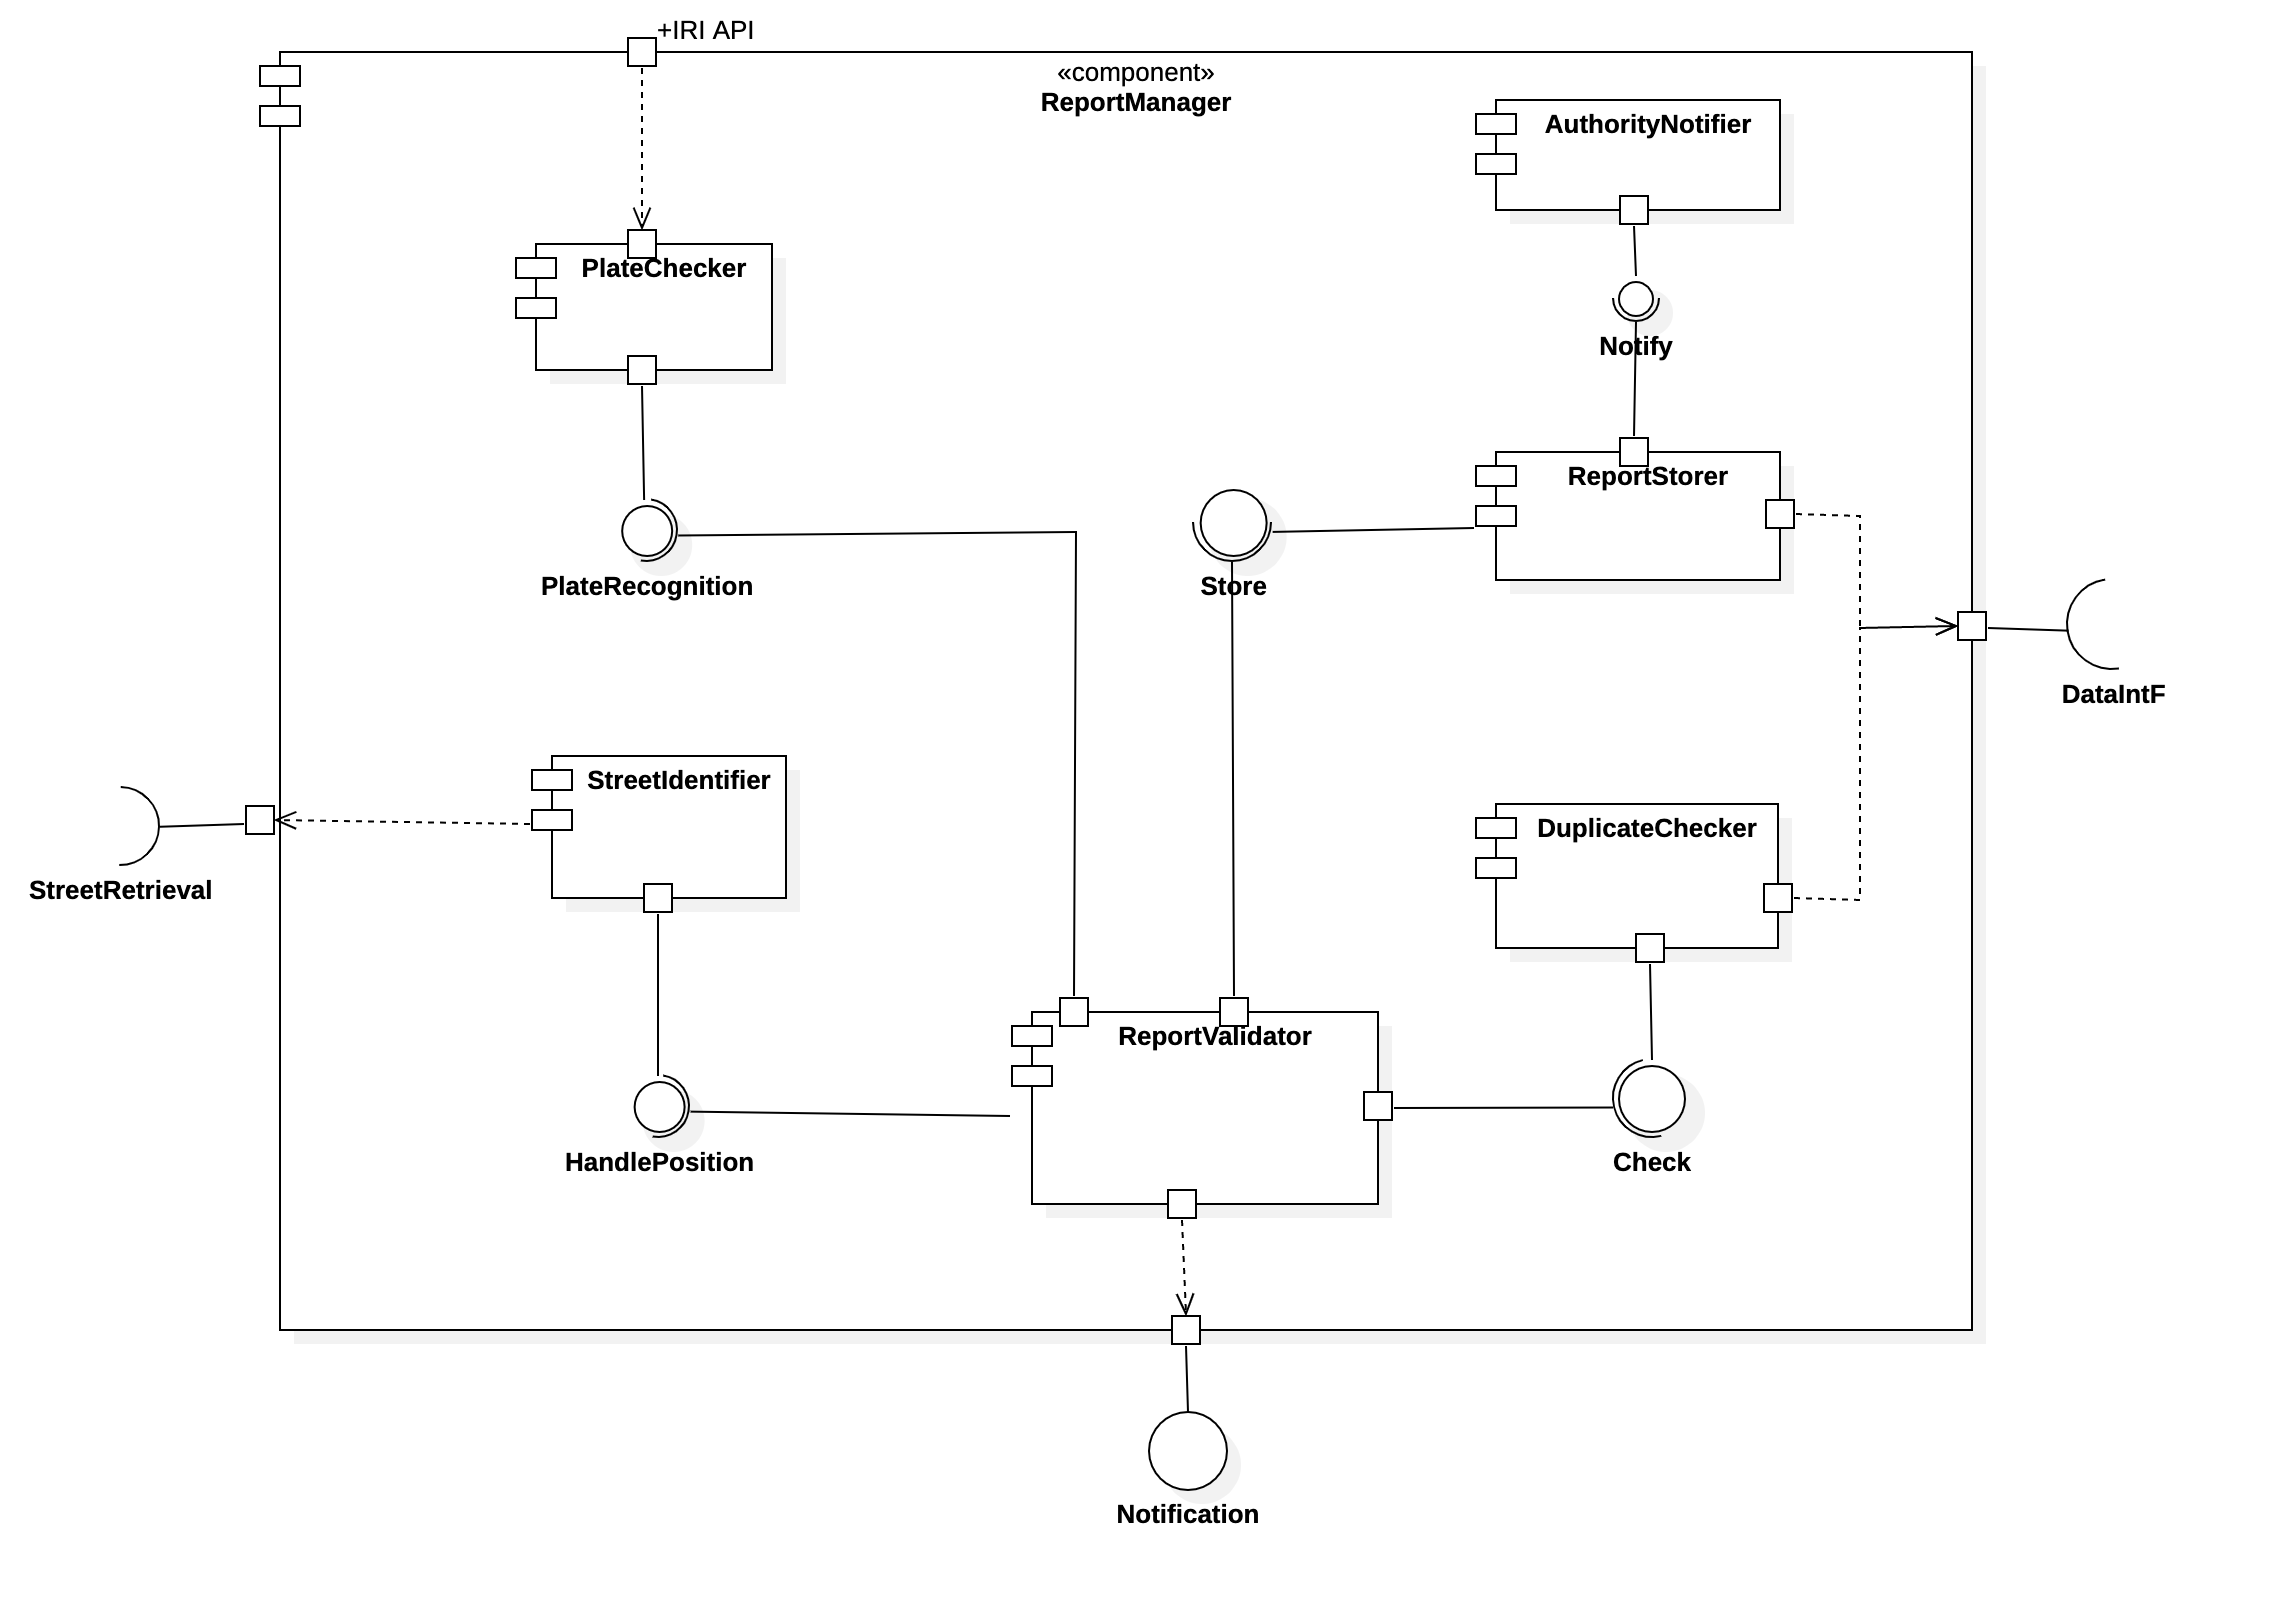
\includegraphics[scale=0.16]{/diagrams/components/reportManager.png}
				\caption{\label{fig:reportManagerComp} Report Manager Component Diagram}
			\end{figure}
		
			\begin{itemize}
				\item \textbf{Street Identifier:} it is the component that manages to retrieve the street where the violation occurred using the GPS position provided in the notification. This component realizes the \textbf{HandlePosition Interface} thanks to the methods provided by the \textbf{StreetsRetrieval Interface} which are the real ones that execute the algorithms provided by the external map management system.
				
				\item \textbf{PlateReader:} it is the component that runs the algorithms provided by the IRI API in order to recognize the plate of the vehicle reported. It realizes the \textbf{PlateRecognition Interface} that is used to benefit of this control, fundamental to validate the notification.
				
				\item \textbf{DuplicateChecker:} it is the component that manages the requests to the notification database in order to determine whether the reported notification is already present or not. It realizes the \textbf{Check Interface} which provides the methods to perform this further control before storing the notification.
				
				\item \textbf{ReportStorer:} it is the component that manages to store the notification once it is ready. It realizes the \textbf{Store Interface} and uses the methods provided by the \textbf{DataIntF Interface} in order to store the data relative to the reporting notification.
				
				\item \textbf{ReportsFinder:} it is the component that deals with the check unread reports functionality, hence the authority-side functionality of the notification process. This component is able to retrieve all the unread reports for the authority that is requesting this functionality. In order to do so it uses the methods provided by the \textbf{DataIntF Interface} providing the query that will be executed whenever an authority requires the check unread reports.
			\end{itemize}
		
		\subsubsection[Map Manager Component]{\hyperlink{toc}{Map Manager Component}}
			\label{sec:mapManagerComponent}
			
			The \emph{MapManager} (\autoref{fig:mapManagerComp}) is the component that deals with all the map issues related to the realization of the functionalities. We have already presented them while describing the MI API (section \ref{sec:componentView}); we are going to see now the components that manage these issues thanks to the methods provided by the external map management system. The specific issue will be managed by the other components using the methods provided by the \textbf{StreetsRetrieval Interface} realized by this component.\\
			
			The components that allow the \emph{MapManager} to handle all the geographical and map issues inside the system are:
			
			\begin{itemize}
				\item \textbf{StreetFinder:} it is the component that allows to retrieve the street where the parking violation occurred once the GPS position is provided. It realizes the \textbf{StreetsRetrieval Interface} thanks to the methods provided by the \textbf{GPS Interface}.
				
				\item \textbf{GPSPositionHandler:} it is the component that runs the algorithms provided by the MI API in order to realize the \textbf{GPS Interface}.
				
				\item \textbf{MapRequest:} it is the component that deals both with the retrieval of the best path between two positions provided by the customer and the mapping of each street with the correspondent safety. The shortest path is managed with the methods provided by the \textbf{Path Interface} while the mapping is carried by the the methods of the \textbf{Map Interface}. It is obvious that for example a request for the unsafe functionality over a path will reflect in a double invocation of the methods realized by this component.
				
				\item \textbf{ShortestPathHandler:} it is the component that runs the algorithms provided by the MI API in order to realize the \textbf{Path Interface}.
			\end{itemize}
			
			\begin{figure}[ht]
				\centering
				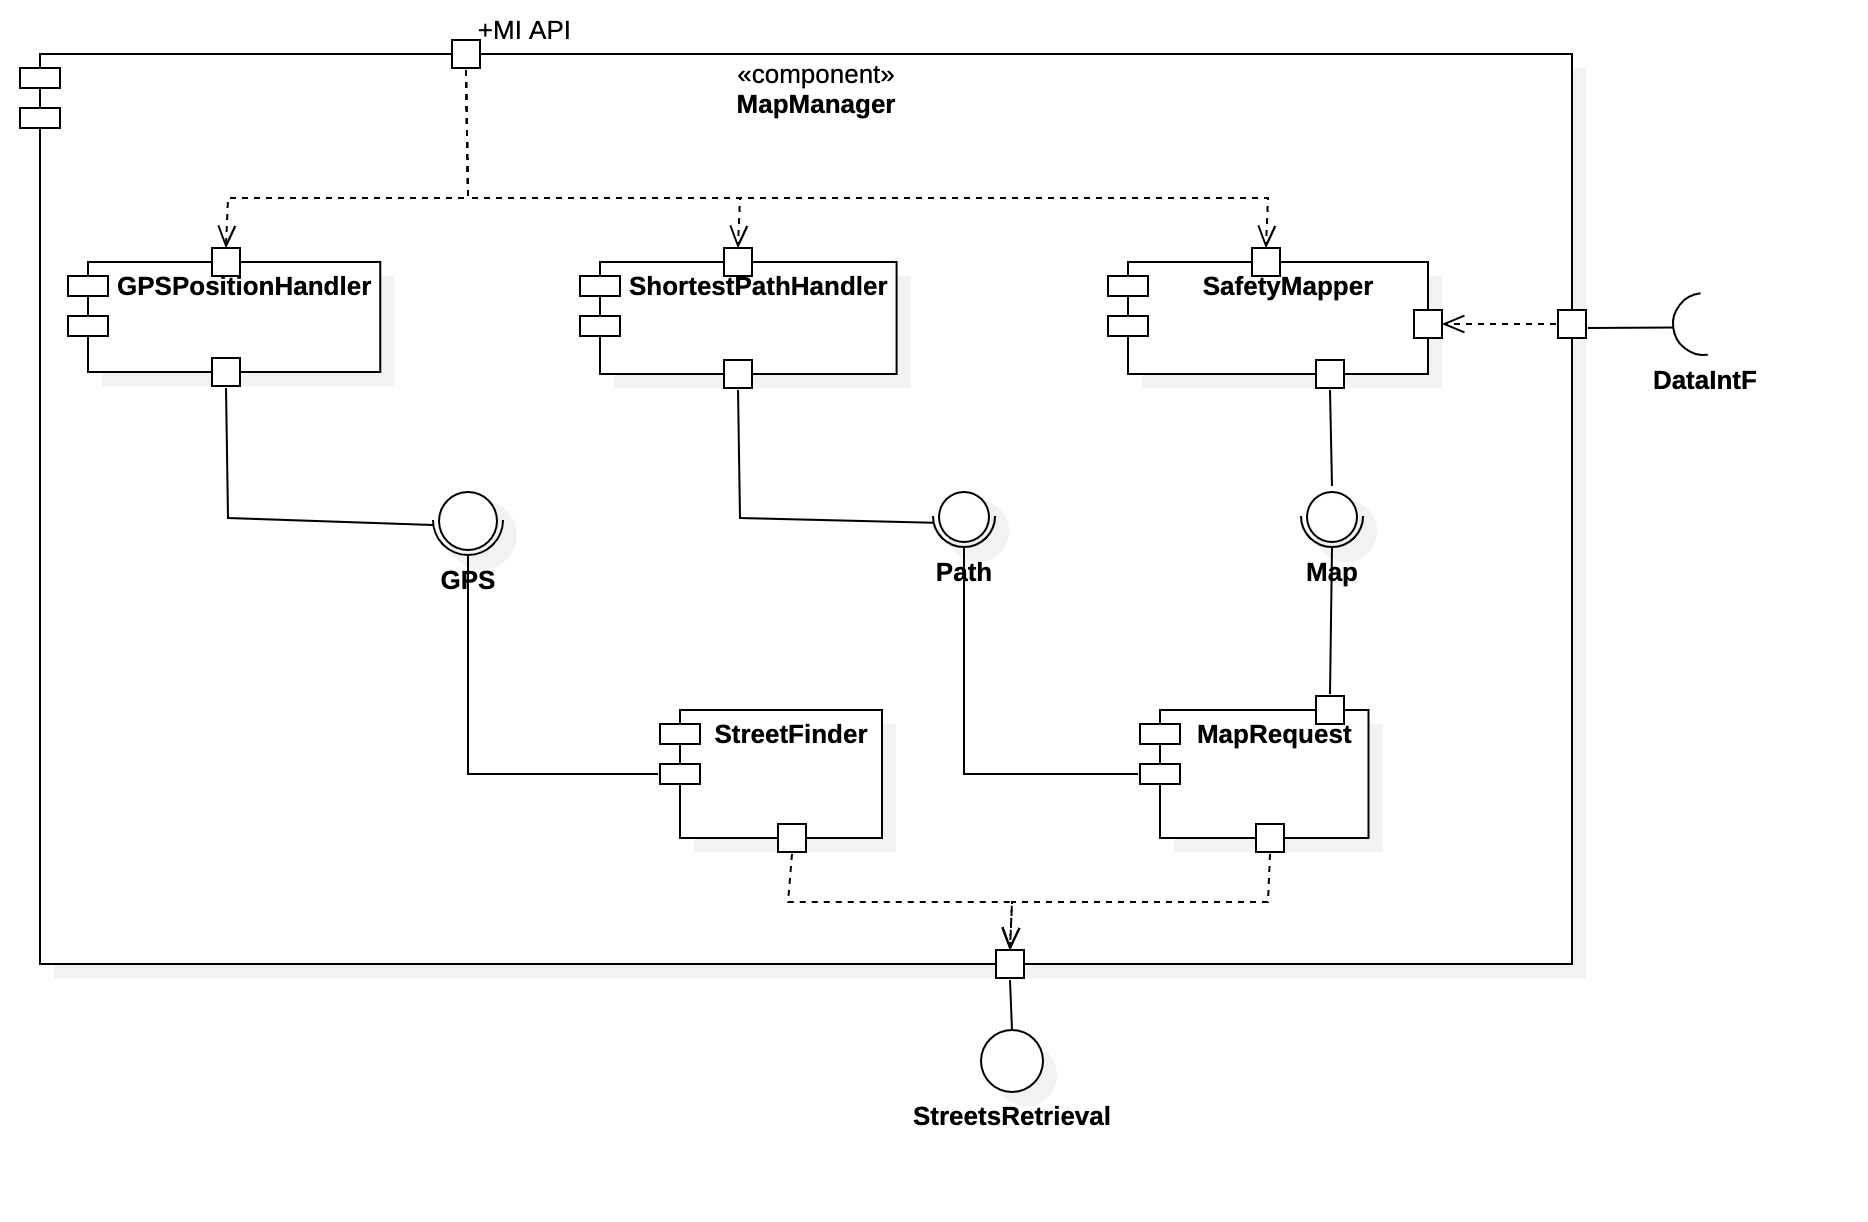
\includegraphics[scale=0.2]{/diagrams/components/mapManager.png}
				\caption{\label{fig:mapManagerComp} Map Manager Component Diagram}
			\end{figure}
		
			\begin{itemize}
				\item \textbf{SafetyManager:} it is the component that runs the algorithms provided by the MI API once it has retrieved all the information about the safety of the streets requested by the customer. It realizes the \textbf{Map Interface} that allows to benefit of the methods that return the data of each street together with its safety in order to be displayed to the client.
			\end{itemize}
		
		\subsubsection[Safety Manager Component]{\hyperlink{toc}{Safety Manager Component}}
			\label{sec:safetyManagerComponent}
			
			The \emph{SafetyManager} (\autoref{fig:safetyManagerComp}) is the component that deals with the safety calculus that has to be carried out every day considering the previous thirty days in order to have the data for the safety functionality. As precisely described in the RASD document \cite{RASD} we have defined a clear way to determine the safety of each street. In order to carry on this calculus we have to consider this component that periodically will run its algorithms in order to update the safety.\\
			
			As we see no interface is provided by this component, in fact, as we have just said it is independent as it needs to run periodically by just retrieving the data over the notifications and accidents and update the safety of the streets.\\
			
			Hence it is important now to describe once more how the safety update works as we can also understand how the components that compose the \emph{SafetyManager} interact in order to obtain its functionality. The system dynamically change, each day the safety of the streets, considering the parking violations data relative of the previous thirty days, thanks to two different kind of tresholds. For each street if at least one treshold is exceeded it means that the street is \textbf{unsafe} otherwise it will be considered \textbf{safe}. The tresholds are:
			
			\begin{itemize}
				\item \textbf{Intervention Treshold:} each intervention is defined with a treshold. On every street every intervention would be possibly chosen as a suggestion. Each type of parking violation or accident, if occurred in a certain street augment the treshold of the interventions linked with that type (hence the same violation or accident may augment at the same time two different interventions). If an intervention's treshold exceeds it means that the street is no longer \textbf{safe} and that its safety has to be updated. In this way counting each day for every street if a treshold for at least one intervention is exceeded allows to determine both the safety of a street but also the possible intervention to be suggested.
				
				\item \textbf{Sum Treshold:} in order to consider also the case where no accident is linked to any intervention (because of the fact we are just considering the parking violations and the accident may be caused by another reason, for example: the speed limit) for each street is also defined another singular treshold that independently from the type determines a street to be \textbf{safe} or not. This treshold augments whenever an accident or a parking violation occurs in the street and thus it is simply determined as the sum of the accidents and parking violations. In this way counting each day for every street if the sum treshold is exceeded allows to determine the safety independently from the type of the accidents that have occurred.
			\end{itemize}
		
			Now that we know better how the safety process works we are able to describe the components that compose the \emph{SafetyManager} in order to provide this functionality:
			
			\begin{itemize}
				\item \textbf{SafetyUpdate:} it is the core component that deals with all the computation related to the calculus of the safety that we have said to happen periodically every day. In order to determine whether an interface is exceeded or not it uses the \textbf{InterventionsSafety Interface} and the \textbf{SumSafety Interface} that allow to determine for a street if one of the tresholds have exceeded. In order to access the data of the reports and the accidents the component uses the \textbf{Reports Interface} and the \textbf{Accidents Interface} to carry out the computation. Hence every day a new block of reports and accidents will be considered in the computation and the oldest one will be discarded, once the safety has been determined the \emph{SafetyUpdate} stores the information thanks to the \textbf{Store Interface} and its functionality will be needed the next day.
				
				\item \textbf{InterventionsManager:} it is the component that realizes the \textbf{InterventionsSafety Interface} providing the methods to determine the safety of a street thanks to the tresholds of the interventions linked to the parking violations and the accidents that occurred in that street.
				
				\item \textbf{SumManager:} it is the component that realizes the \textbf{SumSafety Interface} providing the methods to determine the safety of a street thanks to its sum treshold, by counting the number of parking violations and accidents that occurred in that street.
			\end{itemize}
		
			\begin{figure}[ht]
				\centering
				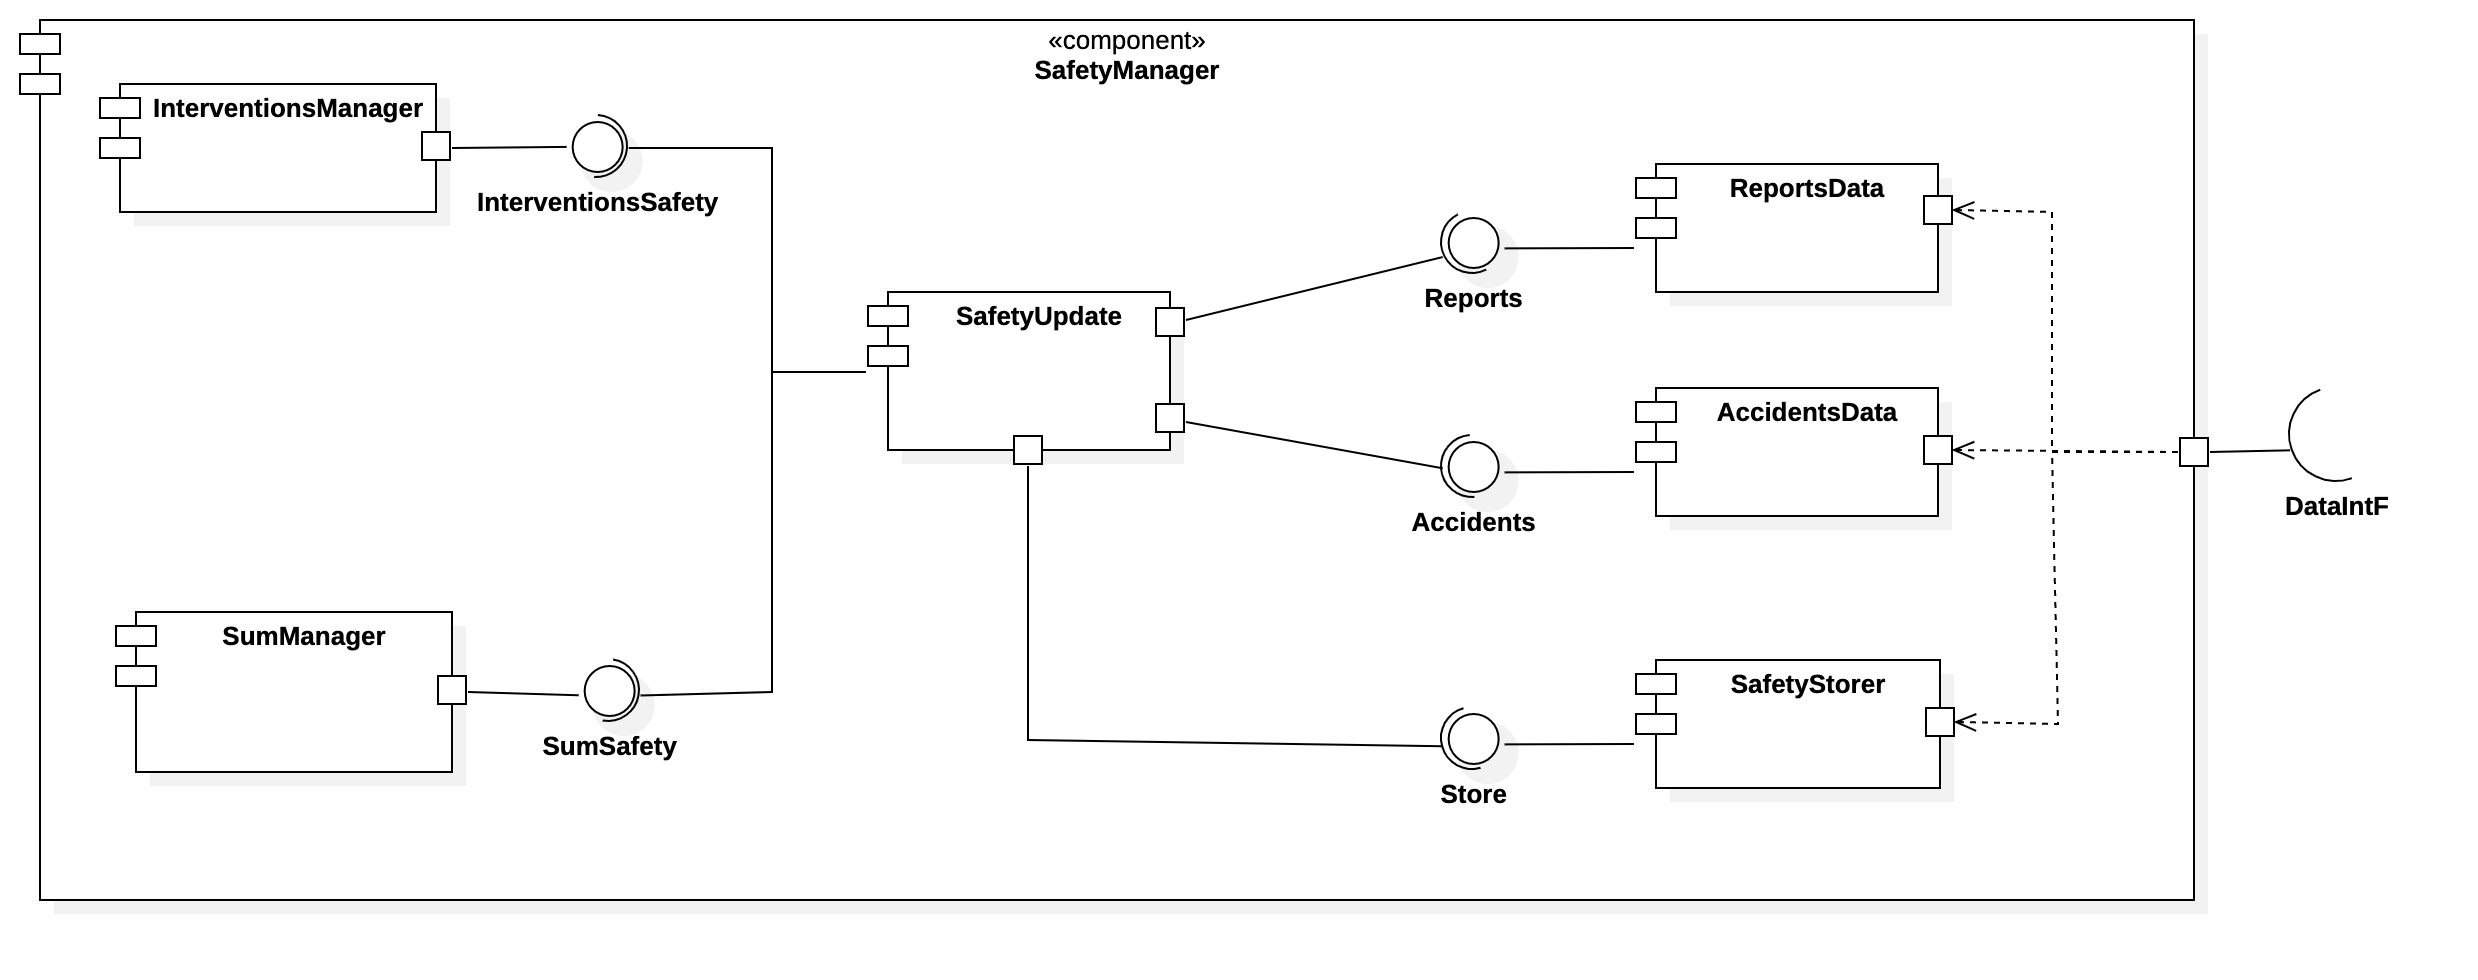
\includegraphics[scale=0.16]{/diagrams/components/safetyManager.png}
				\caption{\label{fig:safetyManagerComp} Safety Manager Component Diagram}
			\end{figure}
		
			\begin{itemize}
				\item \textbf{ReportsData:} it is the component that allows to obtain the information about the type of the parking violations that occurred in a certain street by providing the \textbf{Reports Interface} as they can be considered for the safety update.
				
				\item \textbf{AccidentsData:} it is the component that allows to obtain the information about the accidents that occurred in a certain street by providing the \textbf{Accidents Interface} as they can be considered for the safety update.
				
				\item \textbf{SafetyStorer:} it is the component that is able to store the new information about the safety of each street once is has been updated. It realizes the \textbf{Store Interface} and needs to use the methods provided by the \textbf{DataIntF Interface} in order to complete the storing action.
			\end{itemize}
		
		\subsubsection[Accidents Manager Component]{\hyperlink{toc}{Accidents Manager Component}}
			\label{sec:accidentsManagerComponent}
			
			The \emph{AccidentsManager} (\autoref{fig:accidentsManagerComp}) is the component that deals just with the management of the accidents that have been stored by the authorities over the common interface. As we see only two components are needed, one that receives the accidents by using the methods provided by the \textbf{Authority API} and the other which stores the accidents that have been retrieved.\\
			
			The components that allow the \emph{AccidentsManager} to handle the process of receiving the accidents provided by the authorities thanks to the authority common system are:
			
			\begin{itemize}
				\item \textbf{Accidents Receiver:} it is the component that uses the methods provided by the \textbf{Authority API} in order to retrieve all the accidents that each authority has published. In this way, by updating this type of data periodically as the safety updating process we will be able to have always all the information we need to determine the safety of the streets. Once the accidents data is retrieved this component is ready to store it in the database related to the accidents thanks to the \textbf{Store Interface}.
			\end{itemize}
			
			\begin{figure}[ht]
				\centering
				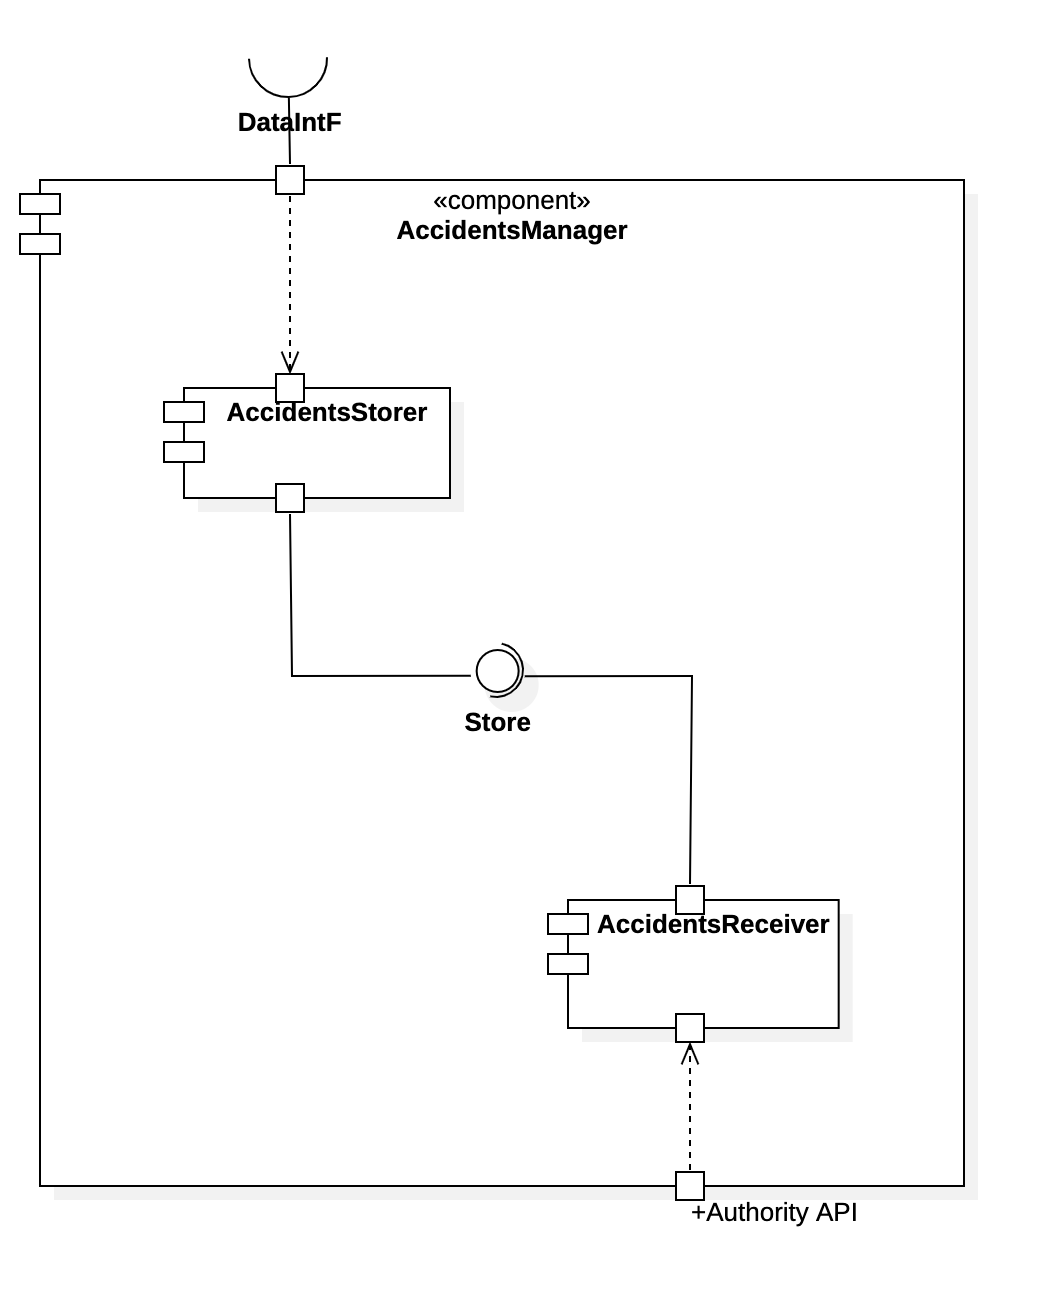
\includegraphics[scale=0.2]{/diagrams/components/accidentsManager.png}
				\caption{\label{fig:accidentsManagerComp} Accidents Manager Component Diagram}
			\end{figure}
		
			\begin{itemize}
				\item \textbf{AccidentsStorer:} it is the component that deals with the storing process of the accidents. It realizes the \textbf{Store Interface} and needs to use the methods provided by the \textbf{DataIntF Interface} in order to store the accidents in the database of the system.
			\end{itemize}
		
		\subsubsection[Data Manager Component]{\hyperlink{toc}{Data Manager Component}}
			\label{sec:dataManagerComponent}
			
			The \emph{DataManager} (\autoref{fig:dataManagerComp}) is the component that deals with all the management of the data needed by the system in order to perform its functionalities. As we can see in the general diagram of the server (\autoref{fig:serverComp}) almost every component needs to use the interface provided by this one in order to provide its functionality.\\
			
			Hence the \emph{DataManager} realizes only the \textbf{DataIntF Interface} which provides the methods for the management of all the information and uses the methods provided by the \textbf{DBMS API} in order to perform on the databases the storing or requesting action needed.\\
			
			The components that allow the \emph{DataManager} to handle all the operations that involve the management of the data stored in the system's databases are:
			
			\begin{itemize}
				\item \textbf{MapManager:} it is the component that provides all the methods that allow to manage the data relative to the map issues, realizing the \textbf{DataIntF Interface}.
				
				\item \textbf{CustomerManager:} it is the component that provides all the methods that allow to manage the data relative to the customers (in particular for the access process), realizing the \textbf{DataIntF Interface}. 
				
				\item \textbf{ReportManager:} it is the component that provides all the methods that allow to manage the data relative to the notification process,hence of all the reports too, realizing the \textbf{DatIntF Interface}.
				
				\item \textbf{InterventionsManager:} it is the component that provides all the methods that allow to manage the data relative to the interventions, realizing the \textbf{DataIntF Interface}.
				
				\item \textbf{AccidentsManagerInterface:} it is the component that provides all the methods that allow to manage the data relative to the accidents, realizing the \textbf{DataIntF Interface}.
			\end{itemize}
		
			\begin{figure}[ht]
				\centering
				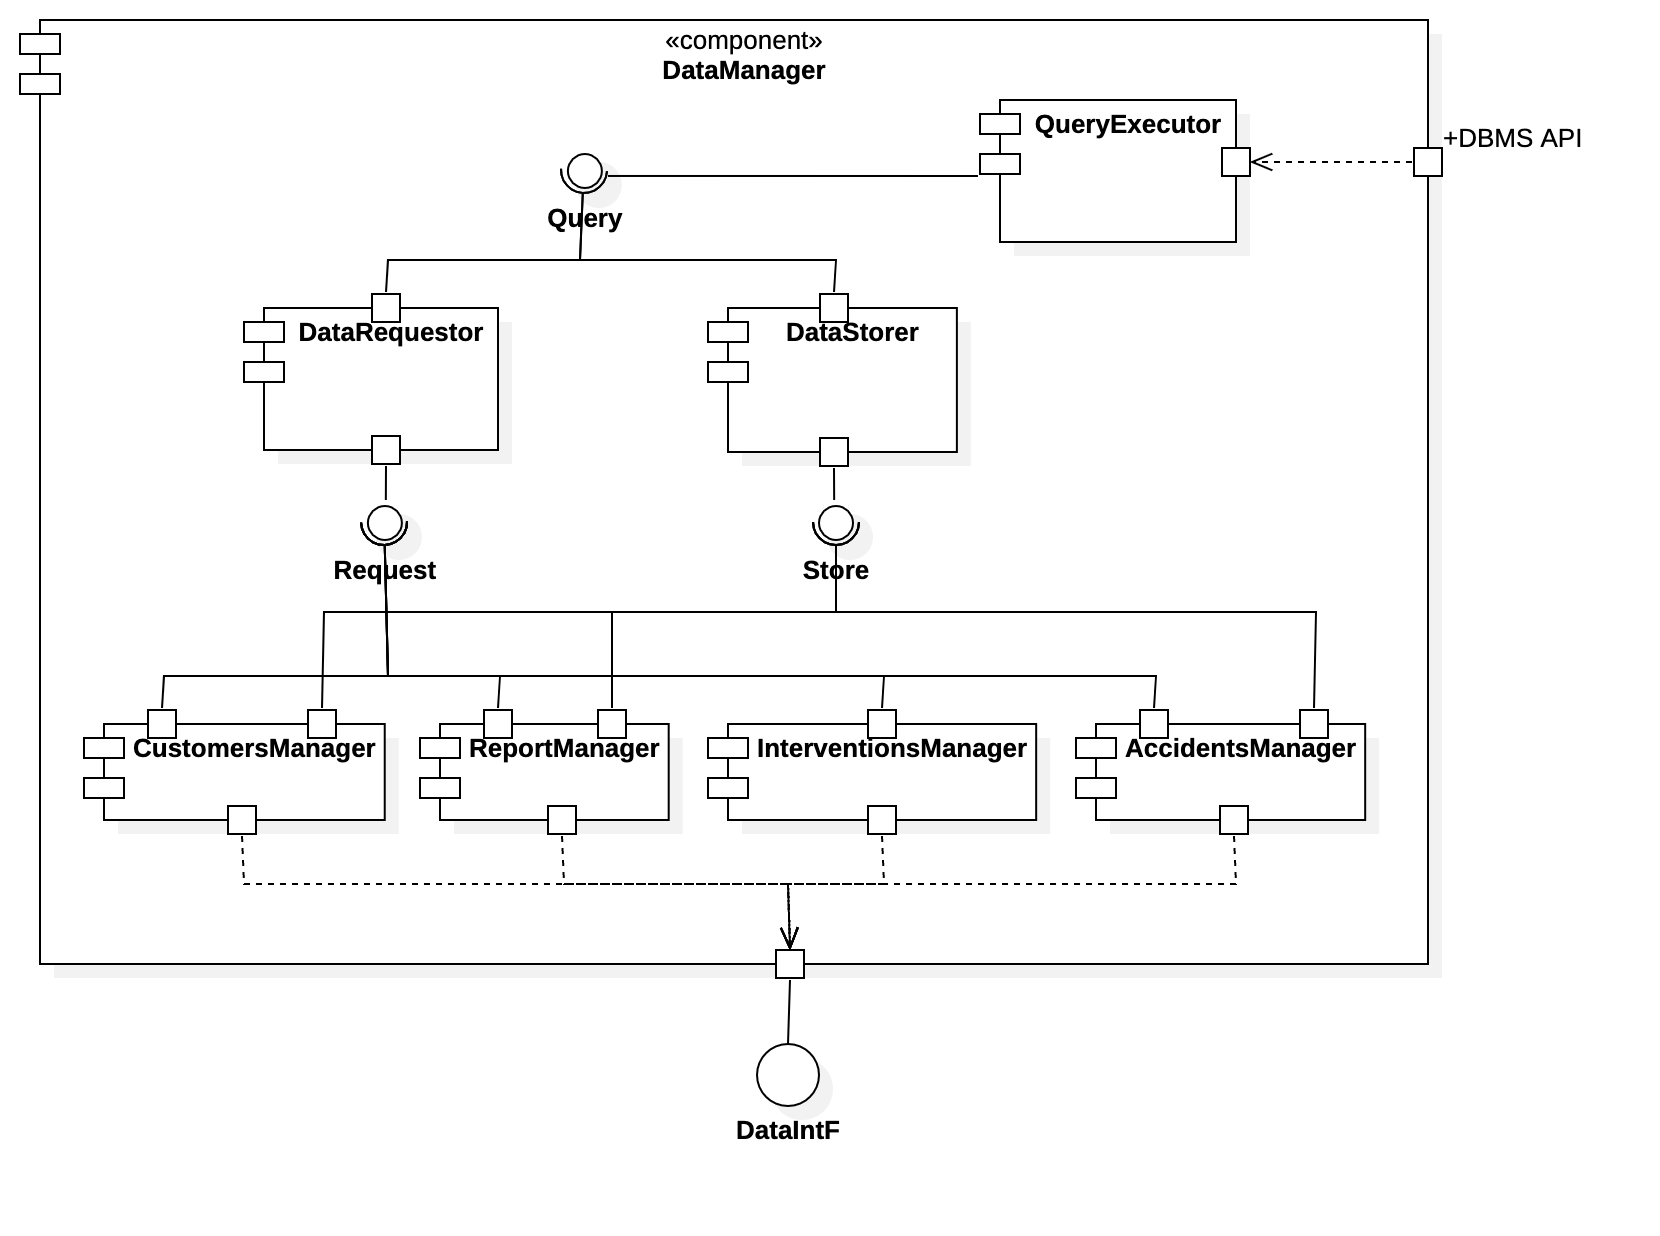
\includegraphics[scale=0.22]{/diagrams/components/dataManager.png}
				\caption{\label{fig:dataManagerComp} Data Manager Component Diagram}
			\end{figure}
		
			\begin{itemize}
				\item \textbf{DataRequestor:} it is the component that allows to build a query that will obtain as a result the information required by one of the managers previously described. It realizes the \textbf{Request Interface} and needs to use the \textbf{Query Interface} in order to execute the query that has been built.
				
				\item \textbf{DataStorer:} it is the component that allows to build a query that will store in the database involved for the information that is going to be stored the data provided. It realizes the \textbf{Store Interface} and needs to use the \textbf{Query Interface} in order to execute the query that has been built.
				
				\item \textbf{QueryExecutor:} it is the component that finally executes the query received either from the \emph{DataRequestor} or the \emph{DataStorer}. It realizes the \textbf{Query Interface} and needs to use the methods provided by the \textbf{DBMS API} in order to manage all the data stored inside the databases of the system.
			\end{itemize}
		
		\subsubsection[Web Server Component]{\hyperlink{toc}{Web Server Component}}
			\label{sec:webServerComponent}
			
			The \emph{WebServer} (\autoref{fig:webServerComp}) is an independent component, out of the server, that deals with the interaction between the web app and the business logic of the system. It realizes the \textbf{WebAppInterface} in order to provide the endpoint for the authorities to access SafeStreet with the web application displayed on their browser. It needs to use the methods provided by the \textbf{WebInterface} in order to establish the interaction between the authorities and the system.\\
			
			The components that allow the \emph{WebServer} to handle the interaction process between the requests coming from the web app and the business logic are:
			
			\begin{itemize}
				\item \textbf{Presentation:} it is the component that deals with the graphical interface that is needed to provide the authorities the access to the system. It realizes the \textbf{WebAppInterface} as it defines all the methods and scripts the browser will use to display the information. In order to manage the interaction it handles the actions performed by the authority with the \textbf{Commands Interface} and sends the requests to the system as they can be processed thanks to the \textbf{Requests Interface}.
			\end{itemize}
			
				\begin{figure}[ht]
					\centering
					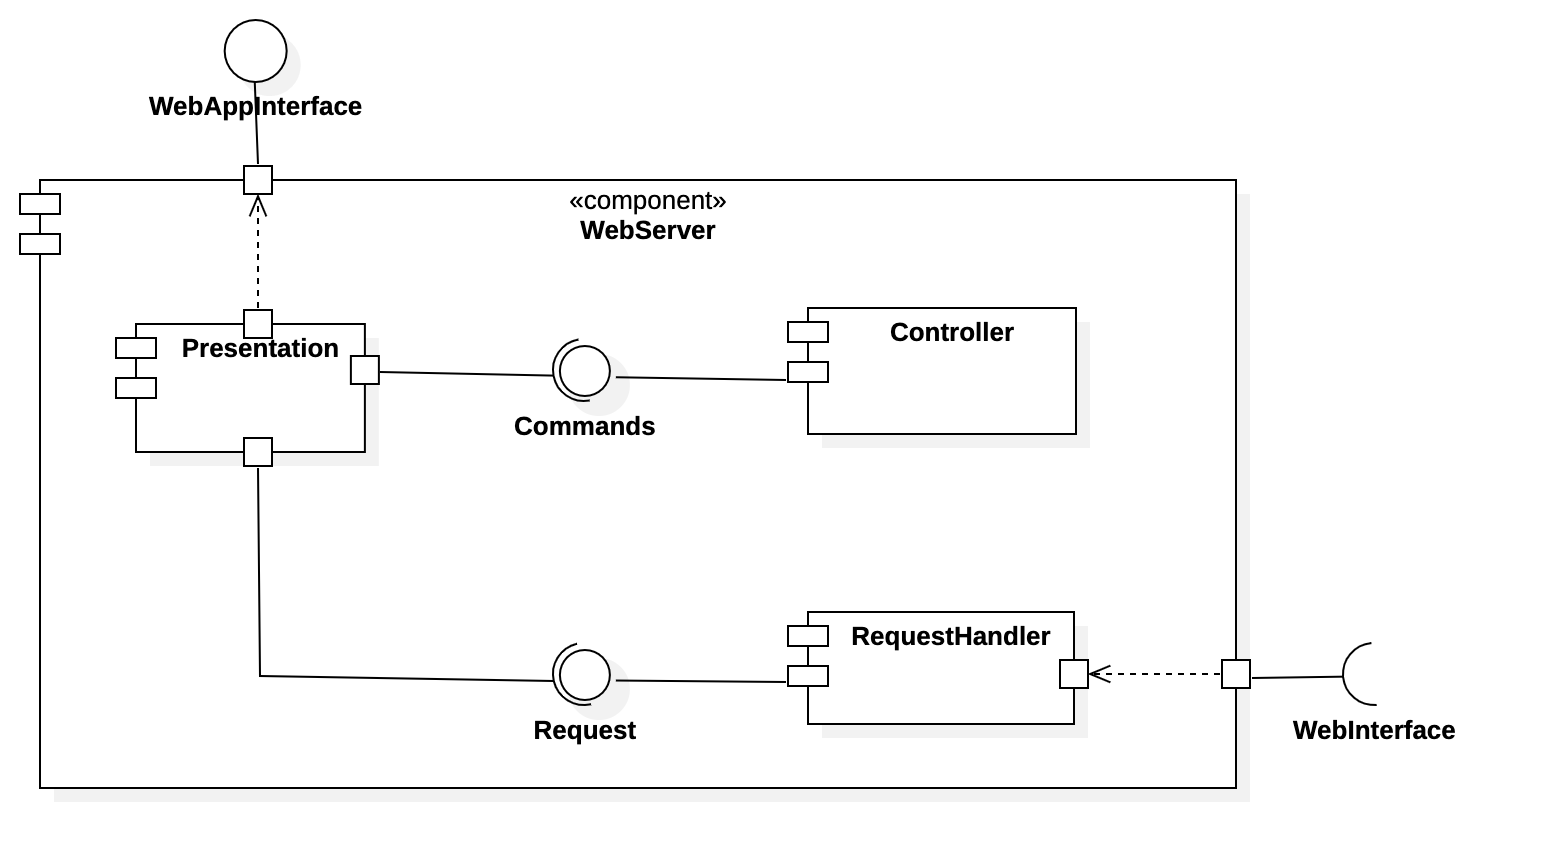
\includegraphics[scale=0.2]{/diagrams/components/webServer.png}
					\caption{\label{fig:webServerComp} Web Server Component Diagram}
				\end{figure}
		
			\begin{itemize}
				\item \textbf{Controller:} it is the component that deals with the logic needed to handle the actions performed by the authority. By providing the \textbf{Commands Interface} it allows to manage the flow of the web application displayed on the browser of the authority.
				
				\item \textbf{RequestHandler:} it is the component that deals with all the requests coming from the web application. Thanks to the \textbf{Request Interface} realized, it is able to process the incoming request and send it to the business logic with the methods of the \textbf{WebInterface} as the functionality required will be displayed in the web application.
			\end{itemize}
		
		\subsubsection[User App Component]{\hyperlink{toc}{User App Component}}
			\label{sec:userAppComponent}
			
			The \emph{UserApp:} (\autoref{fig:userAppComp}) is the other independent component that will be installed on the device of the users in order to provide the interaction with the system. Differently from the \emph{WebServer} this is already the component that will manage the actions performed by the user as it represents the mobile software application. For this reason it only needs to use the methods provided by the \textbf{MobileAppInterface} to send the requests to the system as they can be processed.\\
			
			The components that allow the \emph{UserApp} to handle the interaction process between the requests coming from the mobile app and the business logic are:
			
			\begin{itemize}
				\item \textbf{Presentation:} it is the component that deals with the graphical interface that is needed to provide the users the access to the system. As we have just said the realization of this component is the interface that allows the user to interact with the system; in order to do so it needs to use the methods provided by the \textbf{Commands Interface} and the \textbf{Request Interface}.
			\end{itemize}
			
			\begin{figure}[ht]
				\centering
				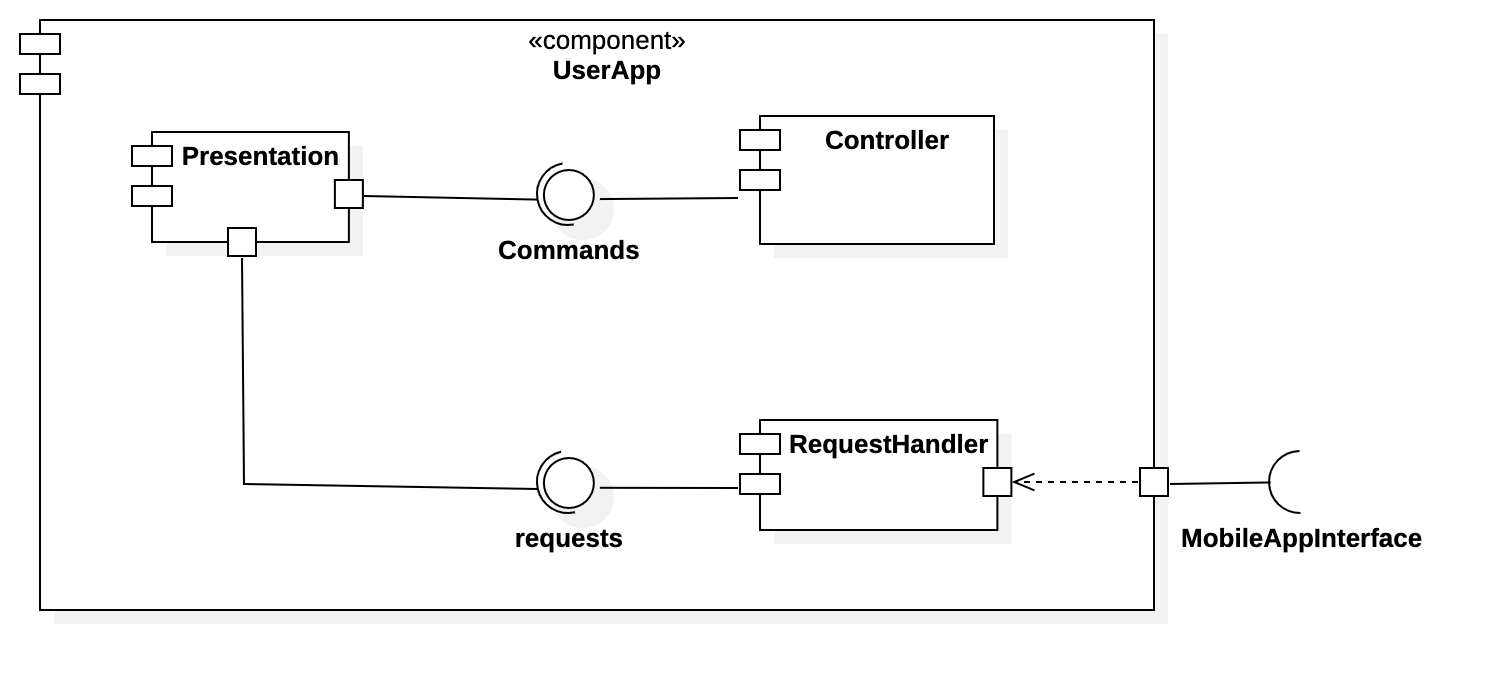
\includegraphics[scale=0.2]{/diagrams/components/userApp.png}
				\caption{\label{fig:userAppComp} User App Component Diagram}
			\end{figure}
		
			\begin{itemize}
				\item \textbf{Controller:} it is the component that deals with the logic needed to handle the actions performed by the authority. By providing the \textbf{Commands Interface} is allows to manage the flow of the mobile application displayed on the device of the user.
				
				\item \textbf{RequestHandler:} it is the component that deals with all the requests coming from the mobile application. Thanks to the \textbf{Request Interface} realized, it is able to process the incoming request and send it to the business logic with the methods of the \textbf{MobileAppInterface} as the functionality required will be displayed in the application.
			\end{itemize}
			
	\subsection[Deployment View]{\hyperlink{toc}{Deployment View}}
		\label{sec:deploymentView}

		As we have seen in the overview (\ref{sec:overview}) and component view (\ref{sec:componentView}) sections, we have designed a system that needs to interact with many agents. In order to define a crowd-sourced application where a lot of information needs to be managed as it can be used to provide different services, we decided to use a \textbf{client-server} architectural approach. As we may have guessed in the high-level component diagram of \autoref{fig:highLevelComp} the business logic is represented by the server component while the clients are designed with two different technologies in order to have the best application software to make the customers interact with the system, depending on their characteristics.\\
		
		The client-side system is composed of:
		
		\begin{itemize}
			\item \textbf{Mobile Application:} for the users
			\item \textbf{Web Application:} for the authorities
		\end{itemize}
			
		Hence, to make this decision possible we need to consider a web server that will manage all the interaction between the web application and the internal system, while we can make directly interface the mobile application with the internal system thanks to the software application installed on the devices of the users.\\
		
		To accomplish the considerations just presented we decided to design the \textbf{client-server} paradigm with a \textbf{four-tier architecture} in order to have a clear separation between the clients and the servers that manage them; the decoupling of the database shown in the composition diagram (\autoref{fig:compositionDiagram}) enforces once more this decision. All the communications between the system and the customers (both users and authorities) are handled via HTTP messages in a RESTful way. All the considerations just reported about some architectural and communication choices will be clearly precised in the devoted section (\ref{sec:selectedArchitecturalStylesAndPatterns}).\\
		
		Let's focus now on the illustration of the four-tier architecture as we can understand how the components that we have previously described are mapped with the tiers of the system. Then in the next section we first illustrate the decision tree we used while designing the system as we can later give the complete description of the deployment of the system.\\
		
		The following picture (\autoref{fig:fourTierArchitecture}) illustrates the tiers of the system needed in order to deploy the components identified in the previous section. 
		
		\vspace{0.3cm}
		
		\begin{figure}[h!]
			\centering
			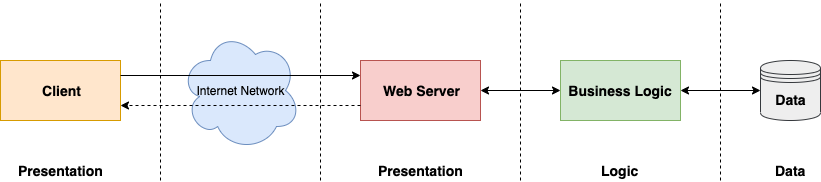
\includegraphics[scale=0.4]{fourTierArchitecture.png}
			\caption{\label{fig:fourTierArchitecture} Four Tier Architecture Diagram}
		\end{figure}
		
		\paragraph{Components Mapping} Now that we know which are the tiers and which are the components we are able to map them together as we can clearly understand how the design is structured before starting with the deployment diagram where we highlight instead which are the devices that run the software components identified.
		
		\begin{itemize}
			\item \textbf{Client:} are the components that allow the interaction of the customers with the system in order to benefit of its functionalities
			
				\begin{itemize}
					\item AuthorityWebApp
					\item UserApp
				\end{itemize}
			
			\item \textbf{Web Server:} it is the layer that allows the interaction between the web application used by the authorities and the system.
			
				\begin{itemize}
					\item WebServer
				\end{itemize}
			
			\item \textbf{Business Logic:} is composed of all the components that allow the computation needed to provide the functionalities of SafeStreets. Hence it is made of all the components inside the server one that are:
			
				\begin{itemize}
					\item ClientHandler
					\item AccessManager
					\item QueryManager
					\item ReportManager
					\item MapManager
					\item SafetyManager
					\item AccidentsManager
					\item DataManager
				\end{itemize}
			
			\item \textbf{Data:} is the layer that deals with the management of all the data needed by the system in order to provide its services.
			
				\begin{itemize}
					\item DBMS
				\end{itemize}
		\end{itemize}
	
		The diagram of next page (\autoref{fig:coloredComponentDiagram}) provides a graphical illustration of what we have just said by coloring with the color of the corresponding layer the components highlighted in the general component diagram already seen.
		
		\newpage
		
		\begin{figure}[htbp]
			\centering
			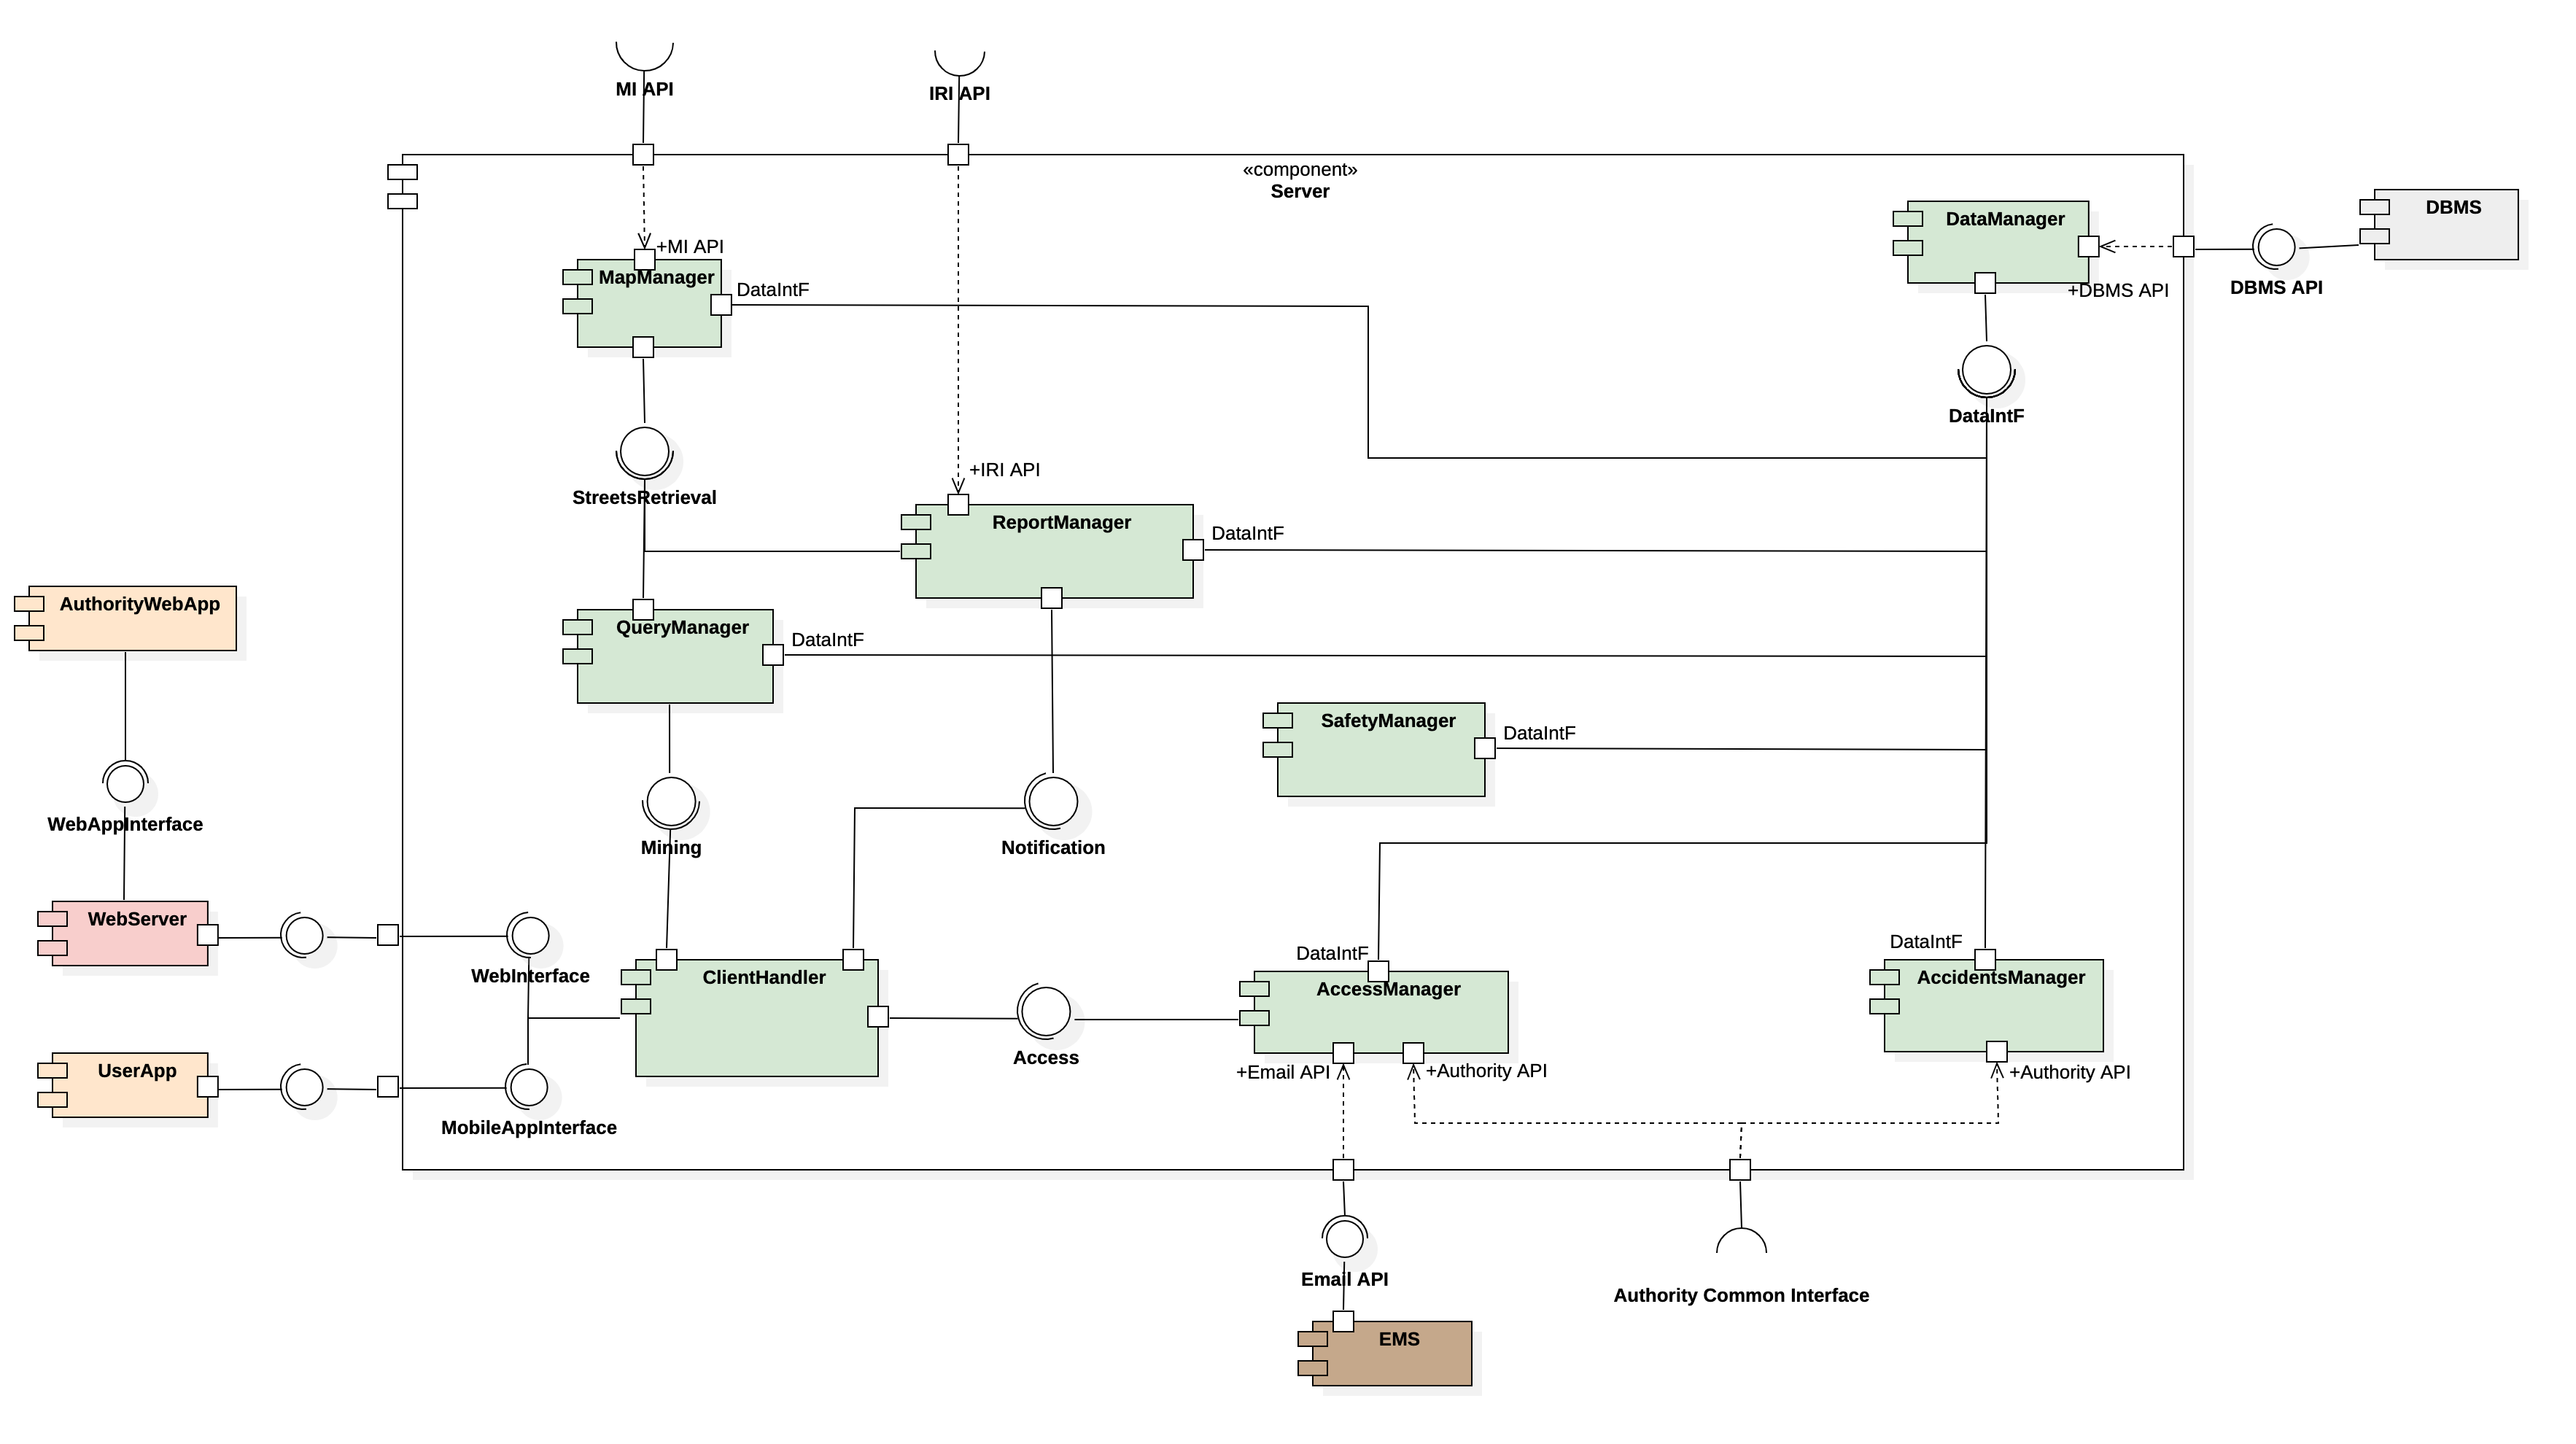
\includegraphics[scale=0.16, angle=90]{coloredComponentDiagram.png}
			\caption{\label{fig:coloredComponentDiagram} Components Mapping Diagram}
		\end{figure}
	
		\FloatBarrier
	
		\subsubsection[Decision Tree]{\hyperlink{toc}{Decision Tree}}
			\label{sec:decisionTree}
			
			Now that we have established how our system is going to be deployed at the highest level possible, before providing the most detailed deployment diagram we present the decision tree we developed while defining the design process as we can justify the diagram of the next section. As we can see in the picture (\autoref{fig:decisionTree}) we started with a \textbf{client-server} decision and then refined with further more detailed decisions.
			
			\begin{figure}[h!]
				\centering
				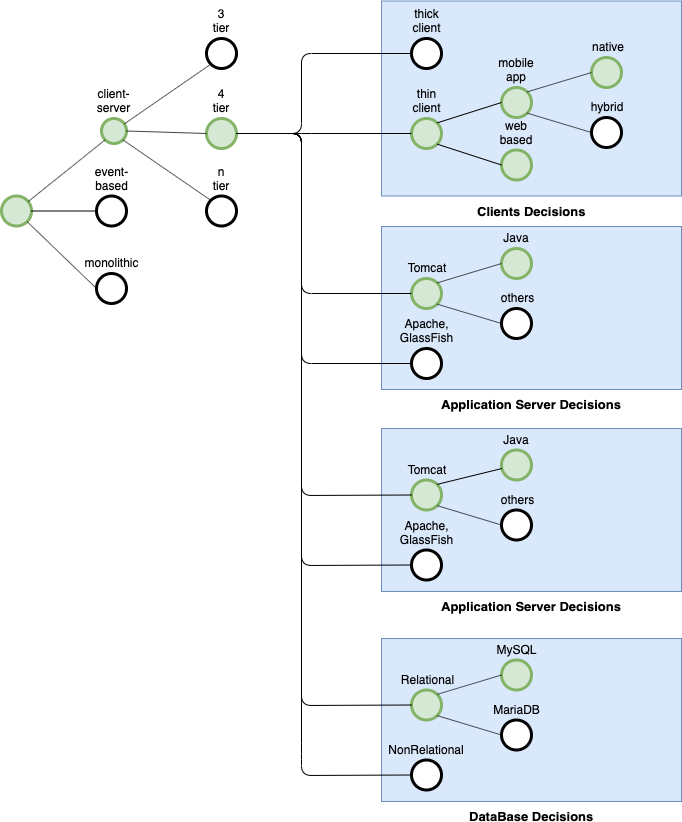
\includegraphics[scale=0.33]{decisionTree.png}
				\caption{\label{fig:decisionTree} Decision Tree}
			\end{figure}
			
		\subsubsection[Deployment Diagram]{\hyperlink{toc}{Deployment Diagram}}
			\label{sec:deploymentDiagram}
			
			In the diagram of the following page (\autoref{fig:deploymentDiagram}) we illustrate a precise description of how and where the components identified are deployed. We still use the colors related to the components now for the nodes that involve them.\\
			
			The communication is presented only between the nodes and not for the components as we already have a precise description of their interfaces that realize their interaction in the component view section (\ref{sec:componentView}). The \textbf{HTTPS} and \textbf{TCP/IP} protocols are used to connect respectively: a connection to a REST API or to a service providing system.\\
			
			All the motivations for the architectural styles and patterns but also the implementation choices that we can see in the picture will be clearly motivated in the devoted section (\ref{sec:selectedArchitecturalStylesAndPatterns}). 
						
			\begin{figure}[hbtp]
				\centering
				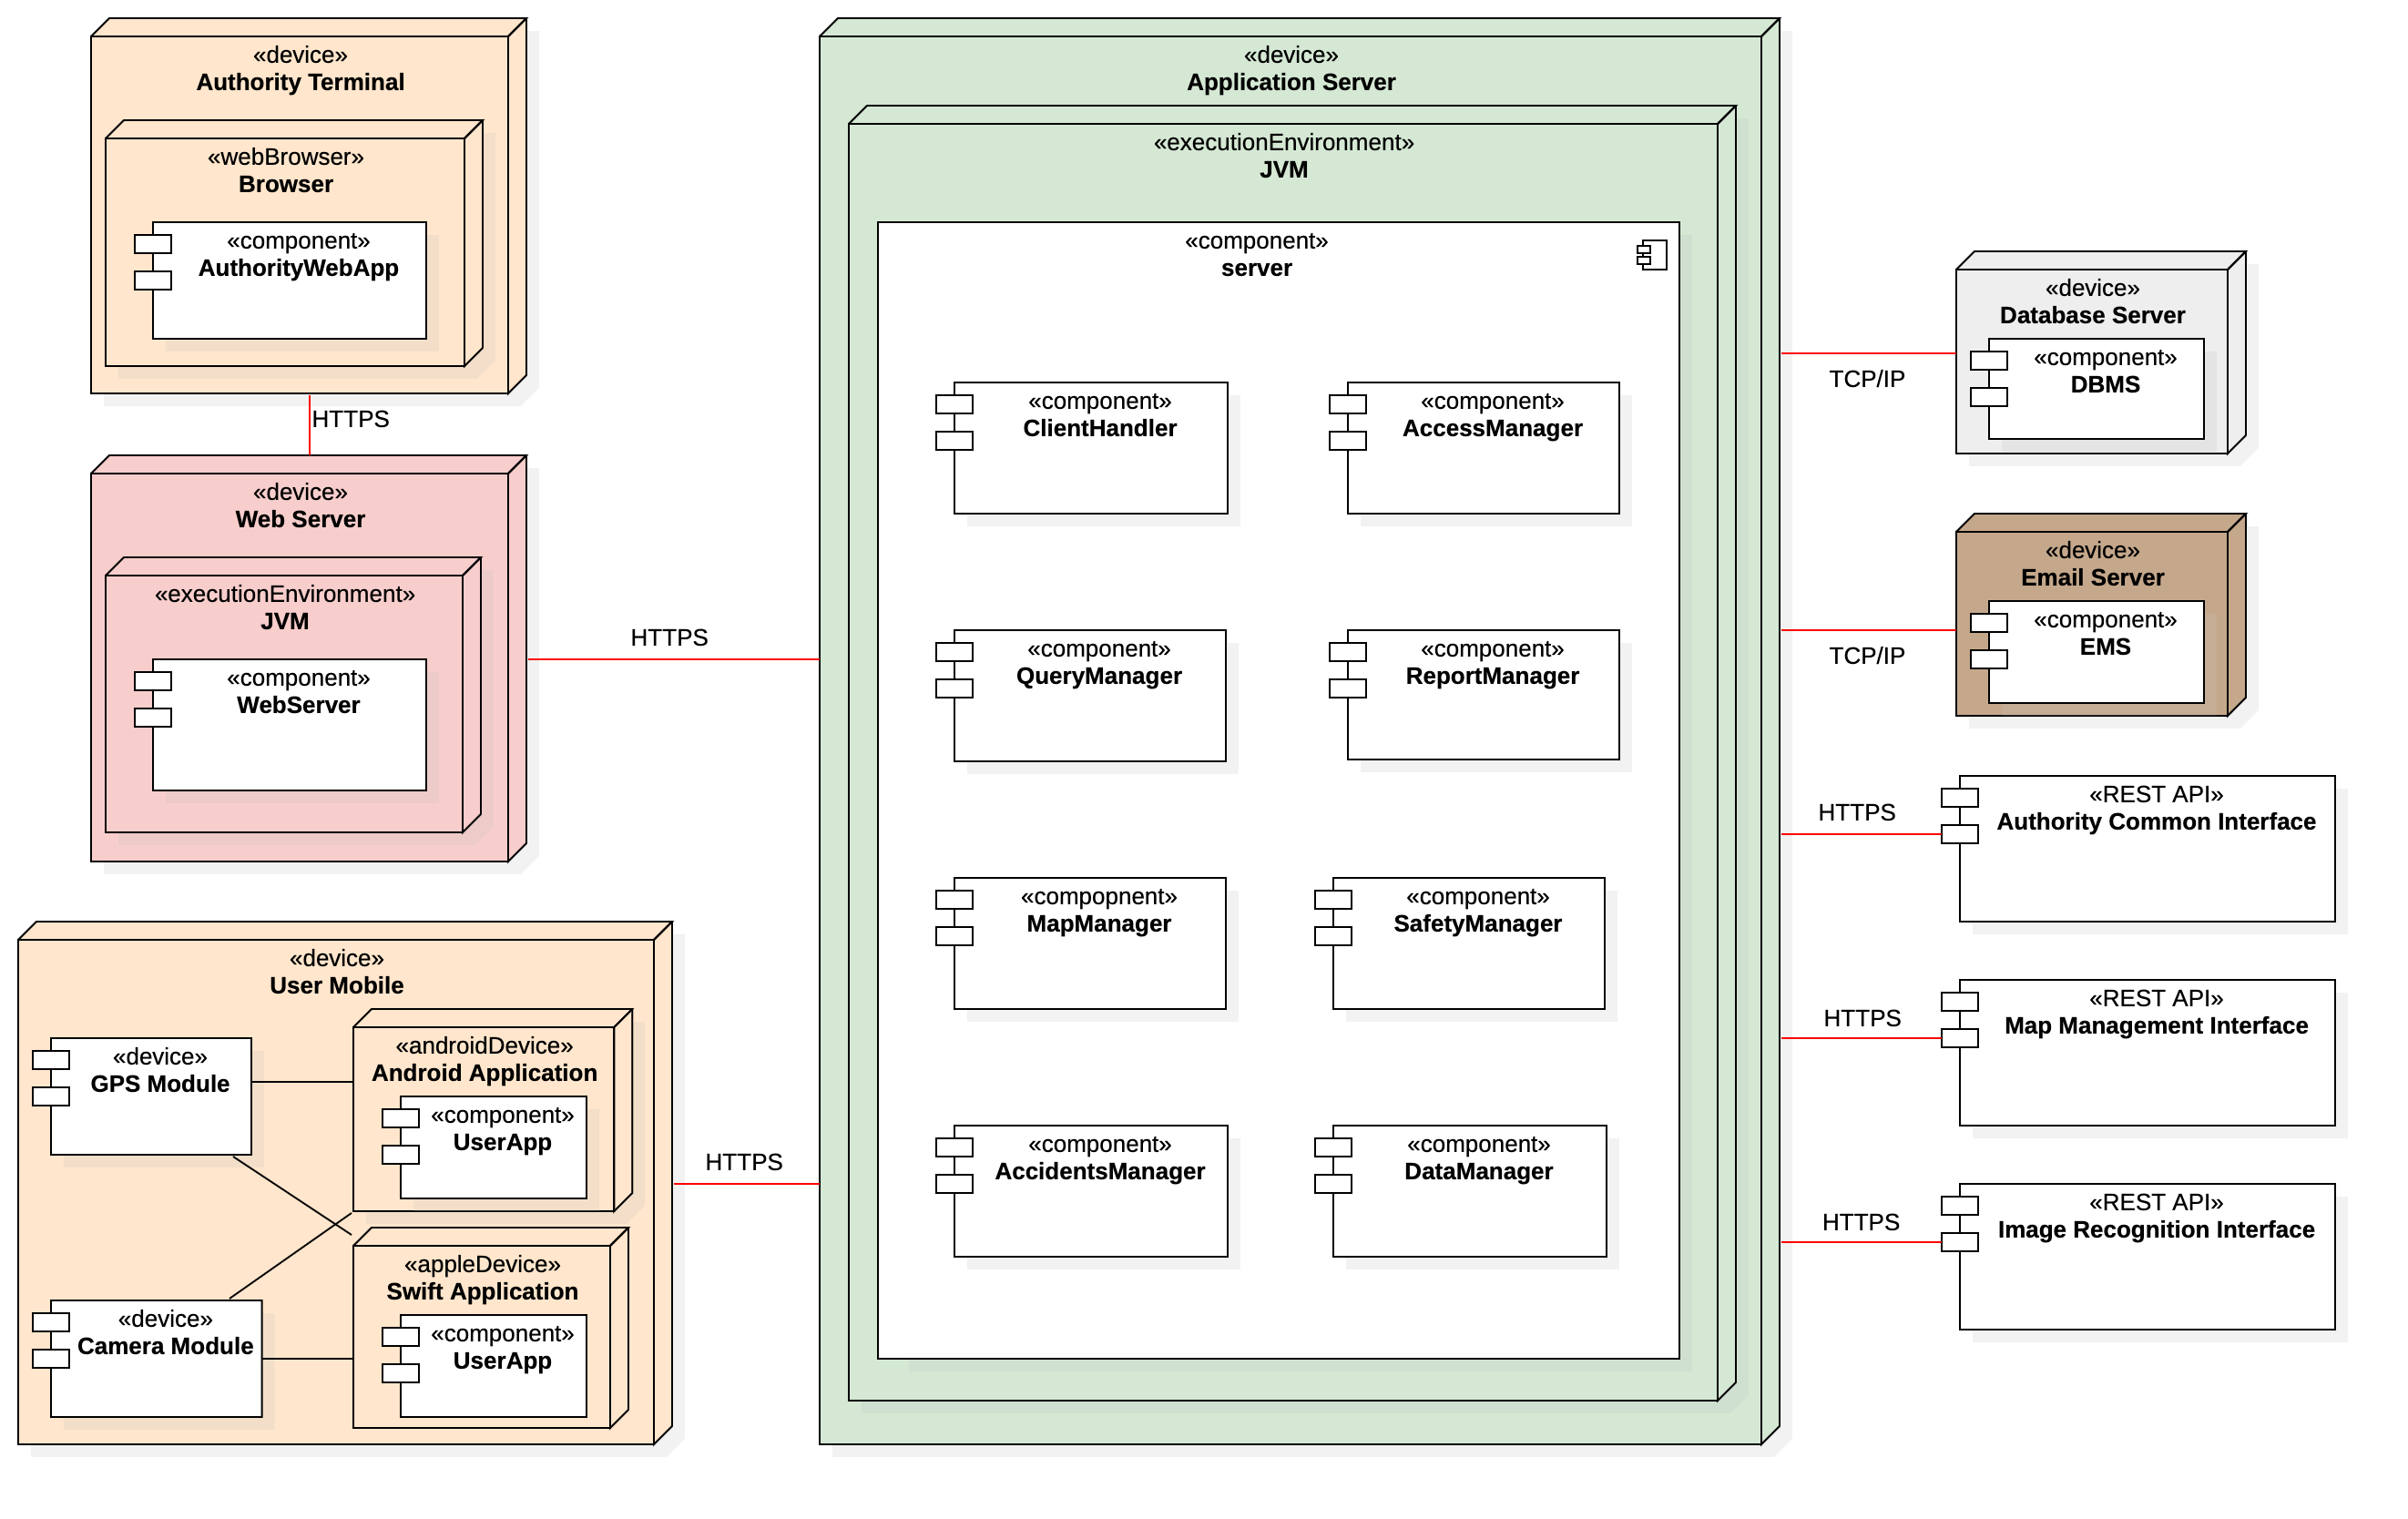
\includegraphics[scale=0.21, angle=90]{/diagrams/deployment/deploymentDiagram.png}
				\caption{\label{fig:deploymentDiagram} Deployment Diagram}
			\end{figure}
		
			\FloatBarrier
			
	\subsection[Runtime View]{\hyperlink{toc}{Runtime View}}
		\label{sec:runtimeView}
		
	\subsection[Component Interfaces]{\hyperlink{toc}{Component Interfaces}}
		\label{sec:componentInterfaces}
		%todo all the APIs go here!
		
	\subsection[Selected Architectural Styles and Patterns]{\hyperlink{toc}{Selected Architectural Styles and Patterns}}
		\label{sec:selectedArchitecturalStylesAndPatterns}
		
		%TODO REST utilizzato per tutte e due in modo da usare la stessa tecnologia, rather than usarne due diverse
		
	\subsection[Other Design Decisions]{\hyperlink{toc}{Other Design Decisions}}
		\label{sec:otherDesignDecisions}						